% Manuscript draft for internal review. Compile with: tectonic main.tex
% Structure: secciones/*.tex (IMRaD), secciones/apendices/*.tex, figuras/png (from figuras/mermaid/*.mmd),
% references.bib (verified metadata), referencias/md (full texts used to check every citation).
\documentclass[11pt,a4paper]{article}

\usepackage[T1]{fontenc}
\usepackage[utf8]{inputenc}
\usepackage{lmodern}
\usepackage{microtype}
\usepackage[margin=2.4cm]{geometry}
\usepackage{setspace}
\usepackage[running]{lineno}
\usepackage{amsmath,amssymb}
\usepackage{graphicx}
\usepackage{booktabs}
\usepackage{tabularx}
\usepackage{longtable}
\usepackage{array}
\usepackage{multirow}
\usepackage{makecell}
\usepackage{enumitem}
\usepackage{xcolor}
\usepackage[most]{tcolorbox}
\usepackage{listings}
\usepackage{pdflscape}
\usepackage{caption}
\usepackage[numbers,sort&compress]{natbib}
\usepackage[hidelinks]{hyperref}
\usepackage{cleveref}

\onehalfspacing
\setlength{\emergencystretch}{3em}
\linenumbers
\setlist{nosep,leftmargin=*}
\captionsetup{font=small,labelfont=bf}
\newcolumntype{Y}{>{\raggedright\arraybackslash}X}
\renewcommand{\cellalign}{tl}

% ---------- Reporting conventions ----------
% \pending{...}: a quantity not yet measured. Never replace with a number that is not in a results JSON.
\definecolor{pendingfg}{HTML}{9A3412}
\definecolor{pendingbg}{HTML}{FFF7ED}
\newcommand{\pending}[1]{\textcolor{pendingfg}{\textsf{[PENDING: #1]}}}
\newcommand{\todoauthor}[1]{\textcolor{blue!60!black}{\textsf{[AUTHOR DECISION: #1]}}}
\newtcolorbox{resultspending}[1][]{colback=pendingbg,colframe=pendingfg,fonttitle=\sffamily\bfseries,
  title={RESULTS\_PENDING},#1}

\lstset{basicstyle=\ttfamily\footnotesize,breaklines=true,columns=fullflexible,frame=single,
  literate={á}{{\'a}}1{é}{{\'e}}1{í}{{\'i}}1{ó}{{\'o}}1{ú}{{\'u}}1{ñ}{{\~n}}1{Á}{{\'A}}1{É}{{\'E}}1
  {Í}{{\'I}}1{Ó}{{\'O}}1{Ú}{{\'U}}1{Ñ}{{\~N}}1{¿}{{?`}}1{¡}{{!`}}1{ü}{{\"u}}1{→}{{$\rightarrow$}}1{—}{{---}}1{…}{{\ldots}}1}

\newcommand{\harness}{multi-call harness}
\newcommand{\mono}{monolithic call}
\newcommand{\formv}{\texttt{form199-v1}}

\title{Monolithic, decomposed and case-model-guided LLM extraction of 199 ICU variables from Spanish
discharge summaries: a paired comparison\\[0.5em]\large Draft for internal review --- not for submission}
\author{\todoauthor{author list, affiliations and corresponding author}}
\date{Draft of 23 September 2026}

\begin{document}
\maketitle

\begin{abstract}
\noindent\textbf{Background.} Large language models (LLMs) can populate structured clinical forms from free
text, but long forms force a design choice that is rarely evaluated directly: request every variable in one
generation, or decompose the form into several calls whose outputs are validated and merged. Independent calls
shorten outputs but lose a common reading of the clinical episode, which many variables require.

\noindent\textbf{Objective.} To compare, on the same patients, models and 199-variable intensive care unit
(ICU) form, three strategies: (A) a single monolithic call; (B) a schema-constrained harness of 18 independent
calls of 2 to 16 variables each; and (C) the same harness in which a preliminary call builds an
evidence-grounded model of the case (ICU stays, timeline, problem status, support, infections, outcome) shared
by all group calls. Outcomes are structural validity, evidence fidelity, cross-block clinical coherence,
agreement with human annotators and cost.

\noindent\textbf{Methods.} Retrospective methodological study on a frozen cohort of 50 de-identified Spanish
discharge summaries from the adult ICU of a public hospital in Chile. All strategies receive the full
line-indexed note, the same annotation rules and the same output contract; evidence is returned as line
identifiers and the quoted text is copied by software. Each strategy is run with three open-weight models on
local infrastructure (Gemma~4 31B, Llama~3.3 70B and Qwen~3.6 35B-A3B) with greedy decoding. The primary
comparison is non-inferiority of B versus A in agreement with a pre-defined human reference in summaries with a
documented ICU stay; C versus B and C versus A are secondary. Differences are estimated within model with a
patient-level paired bootstrap.

\noindent\textbf{Results.} The cohort comprises 50 summaries (median 3 pages and approximately 6{,}000
characters); 12 did not mention an ICU stay and are candidates for exclusion from agreement analyses. At the
23 September 2026 data cut, 63 of 150 planned human annotations had been submitted by 4 reviewers; pairwise
agreement on the 174 boolean variables was $\kappa=0.76$ (95\% CI 0.70--0.82; 19 summaries). In a single-case
pilot with Gemma~4, both A and B returned all 199 variables without truncation; B took 39~min and left 6
relation errors between independently answered groups, and A took 3~h~47~min and was valid after one retry.
Comparative results are \pending{pending the evaluation run}.

\noindent\textbf{Conclusions.} \pending{to be written after the pre-specified analysis. The conclusion must be
limited to the measured paired differences, this cohort, this schema and these three models, and must not
imply clinical use.}

\medskip\noindent\textbf{Keywords:} clinical information extraction; large language models; prompt
engineering; task decomposition; intermediate representation; structured output; discharge summaries;
intensive care; Spanish; evidence grounding; reproducibility
\end{abstract}

\begin{tcolorbox}[colback=gray!5,colframe=gray!50,title=Alternative titles (for author selection),fonttitle=\sffamily\bfseries]
\begin{enumerate}
\item One call, eighteen, or eighteen with a shared case model? A paired evaluation of LLM extraction of a
199-variable ICU form from Spanish discharge summaries.
\item Monolithic, decomposed and case-model-guided extraction of ICU variables with open-weight LLMs: structure,
evidence, coherence and cost.
\item Does sharing a model of the episode make decomposed LLM extraction coherent? A paired study on Spanish ICU
discharge summaries.
\item Auditable extraction of 199 ICU variables with local LLMs: a within-patient comparison of three prompting
strategies.
\item From one long answer to many short ones: decomposition, shared context and cost in LLM form filling from
ICU discharge summaries.
\end{enumerate}
\end{tcolorbox}

\section{Introduction}\label{sec:intro}

Discharge summaries of intensive care unit (ICU) stays condense the clinical history,
organ support, infections, complications and outcome of a critically ill patient into
narrative text. Converting that narrative into the variables of a clinical registry or a
research database still depends largely on manual chart abstraction, which is slow, costly
and difficult to scale beyond small cohorts. Large language models (LLMs) have shown that
clinical information can be extracted from free text with little or no task-specific
training~\cite{agrawal2022fewshot}, and a growing body of work applies them to structured
extraction from clinical notes, pathology reports and radiology reports, including with open-weight
models run on local infrastructure%
~\cite{privacy2024structured,iterativerefine2025,clinicalentityretrieval2024,spaanderman2025structured}.

For research use, the value of an extracted variable depends on whether it can be audited.
A reviewer must be able to see which part of the note supports each answer, to distinguish
a documented absence from a missing answer, and to detect when the output violates the
structure of the form. These requirements become harder to meet as the form grows. When a
single generation must return hundreds of variables, the output becomes long: it may exceed
the token budget and be truncated, it may omit keys or break the JSON structure, and an
error anywhere invalidates or obscures the whole response. A common engineering response is
to decompose the task, for example by processing the note sentence by sentence, by reviewing
and correcting an initial output, by chaining sequential sub-prompts, or by retrieving only the
passages relevant to each variable~\cite{llmie2025,fornasiere2024medical,spaanderman2025structured,clinicalentityretrieval2024}. Decomposition is not
free, however. It multiplies the number of calls, repeats the note in every prompt, increases
latency and creates new opportunities for inconsistency between answers produced
independently for related variables.

Existing studies differ in note type, language, schema size, annotation procedure, models and
metrics, and they rarely isolate the effect of the calling strategy on the same patients, the
same schema and the same models (Section~\ref{sec:related}). In information extraction from
radiology reports, a scoping review found that results could not be compared across studies and
that annotation guidelines, inter-annotator agreement and code were often not
reported~\cite{scoping2024radiology}. The choice between a
single call and a decomposed pipeline is therefore usually made on engineering intuition rather
than on a paired measurement of what each strategy gains and costs.

This study addresses that gap for one concrete and demanding case: a hierarchical annotation form
of 199 variables applied to Spanish discharge summaries of an adult ICU in a public hospital in Chile, the
same form used by human annotators in an annotation platform. We compare three strategies that share the
note, the rules, the output contract and the validator, and differ only in how the form is requested: one
call for all 199 variables; a schema-constrained harness of 18 independent calls, each returning a clinically
coherent group of 2 to 16 variables that is validated, retried on error and merged; and the same harness in
which a preliminary call first builds an evidence-grounded model of the case (ICU stays, timeline, problem
status, support, infections and outcome) that every group call receives. The third strategy addresses a
limitation of independent calls: many variables require inference across the whole episode, and groups that
cannot see each other's answers may reconstruct the clinical story differently. In all strategies the model
cites evidence by line identifier and the software copies the cited text, so that a quotation cannot be
paraphrased or invented by the model.

The contribution is not the use of several prompts, nor the idea of an intermediate representation, both of
which have precedents. It is (i) a controlled, within-patient and within-model comparison of monolithic,
schema-decomposed and case-model-guided extraction under an identical 199-variable contract; (ii) a
reproducible protocol that separates structural validity, evidence fidelity, clinical coherence, agreement
with human annotators and operational cost, and that never converts a failed or truncated answer into a
negative finding; and (iii) an execution with three open-weight models on local infrastructure, with frozen
inputs, hashes and per-call traces.

\subsection{Related work}\label{sec:related}

\paragraph{Single-call structured extraction.} Agrawal et al.\ showed that a general LLM, guided by a one-shot
example in the target format and followed by short deterministic \emph{resolvers}, could extract clinical
information such as medications and their status from English clinical snippets~\cite{agrawal2022fewshot}.
The same work reported two difficulties that bear directly on long forms: it remained ``difficult to guide a
LLM to match an exact schema'' when annotation guidelines span several pages, and prompts specialised for one
status tended to produce an answer even when none was present, a bias toward non-empty outputs. Wiest et al.\
ran Llama-2 models locally on 500 English history sections from MIMIC-IV to extract five binary features,
with an output format in which all features appear in one JSON object~\cite{privacy2024structured}. Unconstrained JSON was ``inconsistent and
defective'', so the authors enforced it with grammar-based sampling; the grammar also forced the model to
write an excerpt before each answer, but excerpts were not checked against the source and a hallucinated
excerpt was reported for the smallest model.

\paragraph{Specification and multi-step pipelines.} Hein et al.\ extracted diagnoses, specimen-level labels and
immunohistochemistry results from kidney-tumour pathology reports with a pipeline of segmentation prompts,
a standardisation prompt and a Python step that produces a long table, refined over six iterations with a
pathologist~\cite{iterativerefine2025}.\footnote{A preprint of the same study was posted under the title
\emph{Prompts to Table}; it reports the same data and results and is not counted as a separate study.} Their
error ontology separated model errors from annotation errors and from insufficient instructions (``schema
issues''); major errors were more frequent in reports with many tests, and no inter-annotator agreement was
measured because the reference was developed iteratively. The study illustrates that the specification of a
long target, not only the prompt, is an object of development and must be reported.

\paragraph{Decomposition strategies compared directly.} Several studies compare a single call with a decomposed
alternative, with heterogeneous tasks and results. In LLM-IE, a sentence-by-sentence extractor achieved higher
F1 than a single whole-document call on three English clinical corpora (for example 0.78 versus 0.44 for event
extraction), mostly through recall, at about twice the GPU time per note; the authors recommend it for ``dense''
tasks and the single call for ``sparse'' ones~\cite{llmie2025}. Fornasiere et al.\ compared zero-shot, few-shot
and sequential prompting with a single 7B model on discharge summaries; sequential prompting did not outperform
few-shot prompting for timeline extraction, and extraction of full medication details remained much harder
than extraction of names~\cite{fornasiere2024medical}. Notably, they supplied the note with numbered rows and
asked the model for the row supporting each extraction, the same principle as the line identifiers used here,
but did not evaluate the correctness of those references. In a preprint benchmark of 15 open-weight models on
Dutch, English and Czech pathology and radiology reports, a manually defined prompt graph of smaller sequential
subtasks gave the largest mean gain over zero-shot prompting ($+12.7\%$), at 37.6~s per report versus 4.5~s for
few-shot prompting; all other strategies requested the whole schema in one JSON call, with at most 22 fields per
template~\cite{spaanderman2025structured}. Finally, CLEAR decomposed the input rather than the output: for each
target variable it retrieved entity-anchored windows and called the model once per window, obtaining higher F1
than full-note input with 71\% fewer input tokens and inference time reduced by 72\%~\cite{clinicalentityretrieval2024}.

\paragraph{Reporting.} A scoping review of 34 studies on information extraction from radiology reports, which
included no generative or prompt-based approaches, found that performance could not be compared across studies
because of differences in data, number of concepts and metrics; 68\% of studies did not mention annotation
guidelines, inter-annotator agreement values were given by 16 of 34, and code was available for 29\%
\cite{scoping2024radiology}. TRIPOD-LLM now asks studies that evaluate LLMs to report prompt development and
its data, inference settings, annotation guidelines, the proportion of multiply annotated data,
inter-annotator agreement, annotator background and compute~\cite{gallifant2025tripodllm}.

\paragraph{Gap.} Across these studies, decomposition has been applied to the input (sentences, retrieved
windows), to the reasoning (segmentation then standardisation, prompt graphs) or to a review pass, and its
reported benefits come with higher cost (\cref{tab:sota}). None of the studies reviewed here compares, on the
same patients and models, a single call with an output-side decomposition by schema group for a form of the
size used here: the largest schema requested in a single call among them has 22 fields, against 199 in this
study. Evidence grounding was either not evaluated or limited to retrieval, and line-numbered evidence, where
used, was not verified. The present study targets that gap with a paired design, verifiable line-level
evidence, full execution logs and open-weight models on local infrastructure.

\subsection{Objectives and hypotheses}\label{sec:objectives}

\paragraph{Research question.} In a fixed cohort of Spanish discharge summaries of patients admitted to an
adult ICU, how do three ways of requesting the same 199-variable form compare when the note, the rules, the
output contract, the validator and the model are held constant: (A) a single call for the whole form;
(B) 18 independent calls, one per group of related variables; and (C) the same 18 calls sharing an
evidence-grounded model of the case built by a preliminary call? The comparison covers structural validity,
evidence fidelity, clinical coherence across blocks, agreement with human annotators and cost, and asks
whether any benefit of the shared case model depends on how much inference a variable requires and on the
quality of the note.

\paragraph{Pre-specified hypotheses.} The following are hypotheses, not findings. H1--H4 were specified
before the pilot for Arms A and B. After the pilot, and before any output was compared with the human
reference, H1 was refined to separate field-level failures from relation violations between groups, H1--H4
were extended to Arm~C, and H5 and H6 were added (Section~\ref{sec:separation}); the original wording is
kept in the protocol history.
\begin{description}
\item[H1 (structure).] Arms B and C have fewer truncated or unparseable outputs and fewer field-level
failures than Arm A. Arm B has more cross-group relation violations than Arm A, because its groups are
answered independently, and Arm C has fewer than Arm B.
\item[H2 (evidence).] Arms B and C have a higher proportion of positive and uncertain answers supported by
valid, relevant evidence lines than Arm A. Because all arms cite by line identifier, literal correspondence
holds by construction; H2 concerns identifier validity, coverage and clinician-judged support.
\item[H3 (agreement, primary).] Arm B is non-inferior to Arm A in agreement with the pre-specified human
reference on the 174 boolean variables of eligible summaries; Arm C is non-inferior to Arm A.
\item[H4 (cost).] Decomposition increases calls, input tokens and total computation per case (A $<$ B $<$ C
in calls and input tokens); latency depends on the inference engine and is reported, not tested.
\item[H5 (clinical coherence).] Arm C violates fewer pre-specified cross-block coherence rules per case than
Arm B.
\item[H6 (inference and note quality).] Arm C improves agreement over Arm B in the blocks that require
inference across the episode (infections, organ failure, complications and ICU discharge), is non-inferior
in medical history, and the improvement is larger in low-quality notes.
\end{description}
A single-case pilot is used only to test the pipeline, the instrumentation and the error handling;
it does not contribute to the estimation of any effect.

\begin{landscape}
\begin{table}[p]
\centering\scriptsize
\setlength{\tabcolsep}{3pt}
\caption{\textbf{Studies used to position this work.} Information as reported by each paper; ``not reported''
means the paper does not state it. IAA, inter-annotator agreement; Source:
\texttt{referencias/INDEX.md} (full texts in \texttt{referencias/md}).}
\label{tab:sota}
\begin{tabularx}{\linewidth}{>{\raggedright\arraybackslash}p{1.7cm}>{\raggedright\arraybackslash}p{2.1cm}>{\raggedright\arraybackslash}p{2.3cm}YY>{\raggedright\arraybackslash}p{2.3cm}>{\raggedright\arraybackslash}p{2.3cm}Y>{\raggedright\arraybackslash}p{1.3cm}Y}
\toprule
Study & Language; notes & Annotators (IAA) & Output schema & Prompt strategy & Models & Evidence validation & Main metric (example) & Code & Main limitation \\
\midrule
Agrawal 2022~\cite{agrawal2022fewshot} & English; clinical snippets, abstracts & 2 authors, adjudicated (no $\kappa$ for new sets) & Free text or lists mapped by resolvers; up to 5 medication attributes & One-shot guided prompts; one item, or medications with status, per prompt & GPT-3 (API) & Resolvers drop tokens absent from input & Medication extraction recall 0.90, precision 0.92 & Data released; code not reported & Hard to match an exact schema; non-empty answer bias \\
Wiest 2024~\cite{privacy2024structured} & English; MIMIC-IV history sections (500) & 3 blinded experts, consensus (no coefficient) & 5 binary features, JSON with excerpt & Fixed prompt with grammar, all features in one JSON (calls per report not stated); zero/one-shot, definitions, excerpt-first & Llama-2 7B--70B, local & Excerpt requested, not checked; hallucinated excerpt reported & Accuracy 0.93--0.96 (70B, zero-shot with definitions) & Yes & English only; lower recall for implicit features \\
Hein 2025~\cite{iterativerefine2025} & Not stated (English excerpts); kidney-tumour pathology reports & Data scientist, statistician, pathologist for ambiguity (no IAA) & JSON to long table; controlled vocabularies & Segmentation then standardisation, per feature or entity class; reasoning passed forward & GPT-4o (API); Llama 3.3 70B, Qwen2.5 72B local & None automated; human discrepancy review & Major error 0.99\%; internal macro-F1 0.99 & Yes & No IAA; no held-out benchmark over all fields \\
Fornasiere 2024~\cite{fornasiere2024medical} & English (+ synthetic Italian); discharge summaries & Challenge gold standards (no new IAA) & Medications (5 fields); dated events & Zero-/few-shot single call; 3-turn sequential; whole vs chunked & Mistral 7B & Row numbers requested, not evaluated & Name F1 up to 0.683; timeline F1 0.790 few-shot vs 0.660 sequential & Pledged, no URL & One model; small datasets \\
Hsu 2025 (LLM-IE)~\cite{llmie2025} & Not stated; i2b2/n2c2 clinical notes & Challenge gold standards & Frames with spans, attributes, relations & Whole document vs per sentence vs review pass; 8-shot & Llama-3.1-70B, self-hosted & Spans in frames; no dedicated verification & Event F1 0.78 per sentence vs 0.44 whole document; $\sim$2$\times$ GPU time & Yes & One model benchmarked \\
Lopez 2025 (CLEAR)~\cite{clinicalentityretrieval2024} & Not stated; clinical notes, radiology reports & 5 physicians, 1 student ($\kappa$ 0.86 and 0.93) & 1 ternary label per variable; 18 variables & Per-variable entity retrieval; one call per retrieved chunk; 5-shot & 5 local models (up to 70B); GPT-4 (Azure) & Retrieval-level only & F1 0.90 vs 0.79 full note; 71\% fewer input tokens & Yes & Multi-chunk prompts and quantisation not tested \\
Spaanderman 2025 (preprint)~\cite{spaanderman2025structured} & Dutch, English, Czech; pathology and radiology reports & Varies by use case (agreement 0.68--0.88 where measured) & Flat JSON, 4--22 fields per template & Zero/one/few-shot, CoT, self-consistency (single call) vs prompt graph & 15 open-weight, 1.5B--685B, local & None evaluated & Prompt graph $+12.7\%$ vs zero-shot; 37.6 vs 4.5~s per report & Yes & No quantisation study; mostly pathology \\
Chen 2026 (two-stage)~\cite{psych2stage2026} & Mostly English; psychiatric discharge summaries (500) & Psychiatrist and NLP researcher, adjudicated ($\kappa$ 0.78) & Sentence events and times; 4 chart-level features & Per-sentence extraction, then one chart-level call on the intermediate list; vs direct and joint & 4 open 8B models, LoRA, local & Source sentence kept; not verified & Onset accuracy 0.73--0.77 vs 0.56--0.65 direct; no gain for counts & Not reported & Single hospital; 4 features \\
Aal Abdulsalam 2026 (multi-agent)~\cite{cancerregistrymas2026} & Not stated; pathology and medical reports (628 evaluated) & Pathologists, senior adjudication ($\kappa$ 0.92) & 6 registry fields, closed labels, evidence quote & Chunking, retrieval, one agent per field, review, aggregation; vs direct prompting & Llama 3.3 70B, local & Quote requested, not checked & Grade F1 0.71$\to$0.78; T and M worse; mean F1 0.71 vs 0.74 & Yes & No ablation \\
Pathak 2026 (preprint)~\cite{promptplanextract2026} & English; lung pathology reports (test 53) & 3 annotators and expert ($\kappa$ 0.81) & 13 CAP fields, JSON & Section mapper, planner metadata injected into parallel field executors, compiler & 5 open models & None & Micro-F1 0.83--0.89 vs 0.96 supervised & Not reported & No single-call baseline or ablation \\
\midrule
This study & Spanish; ICU discharge summaries (50) & 6 assigned, 4 submitting; $\kappa$ 0.76 on current cut & 199 typed variables with hierarchy and exclusions & 1 call vs 18 schema-group calls vs 18 calls sharing a validated case model & Gemma 4 31B, Llama 3.3 70B, Qwen 3.6 35B-A3B, local & Line IDs validated; text copied by software & \pending{paired differences} & Versioned & Single centre; reference incomplete \\
\bottomrule
\end{tabularx}
\end{table}
\end{landscape}

\section{Methods}\label{sec:methods}

\subsection{Study design and reporting}

This is a retrospective, methodological study with a paired, within-patient and within-model
design. Every discharge summary in a frozen cohort is processed by three extraction strategies that
request the same 199-variable form (\cref{fig:architecture}): Arm~A, a single monolithic call; Arm~B, a
schema-constrained harness of 18 independent group calls; and Arm~C, the same 18 group calls preceded
by one call that builds an evidence-grounded model of the case, which is then shared by every group call.
Each strategy is run with three models (\cref{fig:armc} details Arm~C). Strategies are compared within model; models are described side
by side but are not the object of inference, so that strategy and model effects are not confounded.
The pre-registered primary comparison is Arm~B versus Arm~A; Arm~C versus Arm~B, which isolates the
effect of sharing the case model, and Arm~C versus Arm~A are secondary. The study evaluates an
information-extraction pipeline; it does not evaluate a clinical intervention, does not influence
patient care and does not assess a decision-support tool.

Reporting follows the TRIPOD-LLM guideline~\cite{gallifant2025tripodllm}, with the completed checklist
in \ref{app:tripod}. TRIPOD+AI~\cite{collins2024tripodai} informs the description of data,
reference standard and analysis. CONSORT-AI~\cite{liu2020consortai} and
SPIRIT-AI~\cite{rivera2020spiritai} were written for clinical trials and trial protocols; they are used
here only as transparency references, specifically for describing the AI system version, input data,
handling of low-quality or failed outputs, and for registering the analysis plan and its deviations
before outcomes are inspected. The study is not a trial.

\subsection{Setting, data source and eligibility}\label{sec:setting}

The source population consists of 275 de-identified discharge summaries (\emph{epicrisis}) of patients
treated in the adult critical care unit of Hospital Dr.~Sótero del Río, a public hospital in Santiago,
Chile, loaded into a purpose-built annotation platform. The cohort \texttt{concordancia-50-v1} contains 50
of these summaries, fixed on 12 August 2026, before any model output of this protocol was produced. Eligible
summaries were those with a source PDF, parsed sections and a viewer layout, and without any previous
annotation or completed assignment (254 of 275 at selection). They were ranked by the SHA-256 hash of a fixed
seed concatenated with the anonymised identifier, and the first 50 were taken: a reproducible pseudo-random
sample. Each selected summary was assigned to three of five annotator slots, balanced so that every slot
received 30 summaries.

A snapshot of the cohort was exported from the platform database within a read-only, repeatable-read
transaction on 23 September 2026 and, after the de-identification correction described below, again on
24 September 2026; no patient, annotation or assignment was modified. The model
input for each case is the full text of the de-identified document shown in the platform viewer:
the text of the PDF spans that remain after redaction, ordered by position and grouped into visual
lines, with no summarisation. The export used the same redaction implementation and inputs as the
platform endpoint that serves the viewer, and the exported layouts matched the endpoint for all 50
cases. Each text is stored with a SHA-256 hash in a document manifest, the cohort order is fixed in a
list of anonymised \texttt{patient\_id} values, and the snapshot carries a checksum file; the runner
refuses to start if any text, the schema or the manual differs from the frozen version. The 50 summaries
span 144 PDF pages and 9{,}089 text spans (\cref{tab:cohort}).

\paragraph{De-identification check.} A review during the pilot found three defects in the redaction applied
to the first snapshot (23 September 2026): the hospital record number was not masked in 12 of the 50
summaries because it carried an alphabetic prefix; masks of names were applied inside words, cutting
clinical terms (for example a sedative drug name) and one variable key of the human reference; and telephone
numbers written outside the header were masked only by partial coincidence. The redaction rules were
corrected (record numbers with prefix, whole-word masking, Chilean telephone patterns and runs of eight or
more digits except compact dates), verified with synthetic unit tests, and the cohort was re-exported on
24 September 2026 with the same procedure. In the new snapshot all 50 record numbers are masked, no mask cuts
a word, and no telephone-like number or run of eight or more digits remains; the texts differ from the first
snapshot only in 20 summaries and only at masks. All results reported from version~1.3 onwards use the new
snapshot. \todoauthor{deploy the corrected redaction to the annotation platform, re-audit the 275
summaries and describe the de-identification procedure and its audit.} Pattern checks do not amount to an
exhaustive de-identification audit. Redacted segments appear as asterisks and the prompt instructs the
model not to reconstruct them.

\paragraph{Eligibility.} The form describes the first ICU stay, but a summary covers a whole hospitalisation
and the cohort was not screened for the presence of an ICU stay. In the pilot case, an elective surgical
admission, no ICU stay was documented. A lexical screen of the 50 summaries found no mention of the ICU,
the high-dependency unit or intensive care in 12 of them. For such summaries almost every variable is
negative or not applicable by construction, which inflates agreement on trivial negatives. The
pre-specified eligibility criterion for the agreement analyses (H3, H5, H6) is a documented ICU stay,
confirmed by a clinician blinded to model outputs; ineligible summaries remain in the structural and cost
analyses and are reported separately. \todoauthor{confirm the criterion and have the 12 candidate summaries
reviewed.}

\subsection{Annotation form}\label{sec:form}

The target is the annotation form used by human reviewers in the platform (front-end commit
\texttt{42d550f}, schema file SHA-256 \texttt{455fb92f\ldots}). It is a tree of 222 nodes: 23
\emph{mother} categories that organise the form and 199 answerable variables. The 199 variables comprise
174 boolean findings (\emph{leaf} nodes, answered Yes/No/?), 11 dates, 5 single-choice selections
and 9 free-text fields, organised in nine blocks: hospitalisation, medical history (antecedentes),
ICU admission, organ support and interventions, organ failure, infections, complications, ICU
discharge and document quality. Ninety-six variables have at least one boolean ancestor, which
imposes parent--child consistency (a positive child requires a positive parent; a negative parent
forces negative or not-applicable descendants), and 8 variables declare mutual exclusions with other
variables. The mother categories provide context in the prompt but are not scored.

\subsection{Human annotation and reference standard}\label{sec:reference}

\paragraph{Annotation procedure.} Reviewers annotated in the platform, reading the document in one
pane and completing the hierarchical form in the other, following a versioned annotation manual
(manual SHA-256 \texttt{b41b5a58\ldots}; last updated 13 July 2026). For each boolean variable the
reviewer selects Yes (explicit mention, clear synonym or direct unambiguous inference), No (absent in
all relevant sections, negated, or a ruled-out suspicion) or ? (genuinely ambiguous, contradictory or
requiring an unsafe inference). Yes and ? require captured evidence, selected directly from the
document; ? additionally requires an uncertainty level (High, Low, Indeterminate). The manual defines
the unit of annotation as the first ICU stay. Each summary was assigned to three reviewers drawn from
a pool of six. \todoauthor{describe reviewer profile: profession, specialty, years of ICU experience,
training with the platform's interactive examples, and whether reviewers were blinded to each other.}

\paragraph{States kept distinct.} The analysis distinguishes, for every patient--variable pair and
reviewer: \emph{Yes}; \emph{No}; \emph{?} (doubt); \emph{unanswered} (a submitted form in which the item
was left without an answer); \emph{not applicable} (non-boolean fields under a negative parent, or
discharge destination for a patient who died); and \emph{not submitted} (an assignment without a
submitted form). Unanswered and not-submitted items are never treated as No.

\paragraph{Reference definitions (pre-specified).} Because annotation was ongoing at the data cut and
full three-reviewer coverage was available for only one summary, three reference definitions are
pre-specified, in order of priority:
\begin{enumerate}
\item \textbf{Individual reference (primary at the current cut).} Each submitted annotation is
a separate reference. A model output is compared with every submission for the same case; case-level
metrics are averaged over that case's submissions so that each case carries equal weight. Because all
arms are compared with the same references, reviewer noise affects them equally and the paired
differences remain interpretable, although absolute agreement is attenuated.
\item \textbf{Concordant reference (secondary).} For summaries with at least two submissions, an item
enters the reference only if all available submissions agree; items with disagreement are classified
as \emph{unresolvable} and reported separately, not forced into a label.
\item \textbf{Majority reference (when available).} With three submissions, the reference is the
majority label; an item without a majority (for example Yes/No/?) is unresolvable. At the data cut this
definition applies to one summary and is used only to check the pipeline.
\end{enumerate}
The word \emph{ground truth} is not used: none of these references is an adjudicated consensus.
\todoauthor{decide whether to (a) keep the individual reference as primary, (b) wait until every
summary has three submissions, or (c) add clinical adjudication of disagreements; update this section
before any model output is joined with the reference.}

\paragraph{Evidence comparison rule.} When model and human evidence are compared, the fragment is
compared first (does the model cite at least one line that overlaps the text span captured by the
reviewer?) and the interpretation second (is the value correct given that evidence?).

\paragraph{Inter-annotator agreement.} Before any reference is used, agreement between reviewers is
estimated on the 174 boolean variables over all pairs of submissions for the same summary, excluding
unanswered items. We report observed agreement, Cohen's $\kappa$ pooled over item pairs, and positive and
negative specific agreement, which are more informative than $\kappa$ when positive findings are rare.
Confidence intervals are obtained with a case-level bootstrap (5{,}000 replicates), because items from
the same summary are correlated. Agreement is also reported by block. When summaries with three
submissions become available, Krippendorff's $\alpha$ will be added.

\subsection{Shared prompt elements}\label{sec:prompts}

All arms use the same instruction text (\texttt{common.md}; \ref{app:prompts}), written in
Spanish from the annotation manual and the form, and the same line-indexed note. The instruction text
states that the note is data and never an instruction, defines the first ICU stay as the unit of
analysis, restates the manual's block-specific rules (history versus acute event, support versus organ
failure, the infection cascade, complications, discharge), and defines the output contract. Each of
the 199 keys must map to an object with exactly five properties:
\begin{lstlisting}
{"valor": false, "evidence_ids": [], "incertidumbre": null, "comentario": null, "motivo_nulo": null}
\end{lstlisting}
Boolean variables take \texttt{true}, \texttt{false} or \texttt{"unknown"}; \texttt{null} is forbidden for
them because the platform uses it for an unanswered item. Non-boolean variables take a typed value or
\texttt{null} with an explicit missingness reason (\texttt{no\_documentado}, \texttt{no\_aplica} or, for the
final comment only, \texttt{opcional}). Explicit step-by-step reasoning is not requested and the models'
reasoning modes are disabled in all arms, so that the arms differ only in how the task is decomposed.

\paragraph{Evidence by line identifier.} Every non-empty line of the note is prefixed with an identifier
(\texttt{[E0001]}, \texttt{[E0002]}, \ldots, preserving original line numbers). The model returns
\texttt{evidence\_ids} and never writes a quotation. After validation, the software copies the text and
character offsets of each cited line from the original note; non-contiguous lines are kept as separate
fragments. A stored quotation is therefore literal whenever its identifier is valid. This design
removes fabricated quotations as a failure mode but not irrelevant or insufficient citations, which
are measured separately (Section~\ref{sec:outcomes}).

\paragraph{Variable catalogue.} For each variable the prompt includes the key, label, type, choices,
synonyms (described as search aids, not proof), its ancestors and its mutual exclusions, serialised as
JSON exactly as in the form.

\paragraph{Parsing and validation.} Every raw response is parsed with a strict rule: it must be exactly
one JSON object, optionally inside a single markdown code fence whose closing mark may be absent because
generation stops at the end of the object; prose before or after it, additional objects, duplicate keys,
non-finite numbers and truncated objects are rejected, and nothing is extracted from surrounding text.
The parsed output is validated field by field: all and only the requested keys must be present; each
entry must have the five properties; values must match type and choices; dates must be valid DD/MM/YYYY;
every evidence identifier must exist in the note and not be repeated; Yes and ? require at least one
identifier; ? requires an uncertainty level; documented non-boolean values require evidence except the two
subjective quality fields. A rejected or invalid response triggers up to two retries that receive the
errors and the previous output (or the raw response, if it could not be parsed). Failed or missing answers
are never imputed as No. Each attempt writes a trace with the exact prompt, raw and parsed output, errors
and inference metadata.

\subsection{Arm A: monolithic call}\label{sec:mono}

Arm A requests the 199 variables in one call: the instruction text (with the group-specific sentence
replaced by a statement that the whole form is requested), the concatenation of the 18 group catalogues
in the same order, and the indexed note. The output is validated against all 199 fields and the
cross-variable relations in a single pass, and a retry regenerates the complete form. The monolithic
prompt has 114{,}338 characters before the note. Arm A is implemented as a separate module
(\texttt{monolithic.py}) so that the code hashes that sign Arm B outputs are unchanged; its signature adds
the module hash, the strategy and the output budget.

\paragraph{Output budget.} An entry with empty evidence already serialises to about 100 characters, so a
complete answer requires roughly 20{,}000 characters before any evidence identifier or comment; a budget of
4{,}096 new tokens, adequate for a group of 16 variables, would decide the comparison by construction. The
primary analysis gives Arm A 16{,}384 new tokens, within the context window of the three models (131{,}072
tokens for Llama~3.3 and 262{,}144 for Gemma~4 and Qwen~3.6), and a sensitivity analysis uses the per-call
budget of Arm B (4{,}096 tokens) to quantify truncation attributable to the budget alone.

\subsection{Arm B: schema-constrained multi-call harness}\label{sec:harness}

The 199 variables are partitioned, in form order and within block, into 18 groups of at most 16
variables (sizes 2 to 16; \cref{tab:groups}). The partition is mechanical (consecutive variables within
a block) and was not tuned on outcomes. Each group call receives the instruction text, the group catalogue
and a closing sentence stating that the split is technical and that the whole note must be read; the
full indexed note is sent in the user turn (\cref{fig:harness}). The 18 calls are independent: a group
does not see the answers of other groups. Each group is validated and retried on its own; a group that
remains invalid is recorded as failed and its variables are missing. Checkpoints signed with a hash of the
protocol, runner and inference code, model, case and generation settings allow an interrupted job to
resume only validated groups produced under an identical configuration.

After the 18 groups, the merged output is validated as a whole, adding cross-variable relations:
parent--child consistency, mutual exclusions and the rule that a deceased patient has no discharge
destination. Of the 137 parent--child relations between variables, 51 link variables in different groups,
as do 3 of the 7 mutual-exclusion pairs. Relations that span groups cannot be repaired by the per-group
retry and are reported, not silently corrected; a case with any remaining error is marked
\texttt{valid=false}.

\paragraph{Unit of validation and partial outputs.} The unit of validation is the group in Arms B and C
and the form in Arm A. When a unit remains invalid after retries, Arms B and C keep no answer from that
group, whereas Arm A keeps the individual fields of its last attempt that pass every field-level check.
Because this asymmetry favours Arm A in variable-level validity, that outcome is computed in all arms with
the same field-level rule (using the last attempt of failed groups) and, as a sensitivity analysis, with
each arm's own unit rule.

\subsection{Arm C: harness with a shared case model}\label{sec:armc}

\paragraph{Rationale.} Several variables require inference across the whole episode rather than the reading
of a single sentence: the boundaries of the first ICU stay, whether a condition was chronic or acute,
whether organ support accompanied organ failure, and the chain from infection to sepsis, organ failure and
outcome. In Arm~B each group reconstructs that story on its own and cannot see what other groups decided;
the pilot showed the consequence, with dates of mechanical ventilation answered as undocumented in one group
while another group had established that ventilation did not occur. Arm~A sees the whole form but must hold
199 definitions and generate a long output in one pass. Arm~C tests a third option: build an explicit,
verifiable representation of the episode once and give it to every group. The design follows established
ideas: a shared structure read by independent specialists, as in blackboard architectures%
~\cite{erman1980hearsay,nii1986blackboard,blackboardmas2025}; a first pass that plans the answer and a second
that expands its parts in parallel~\cite{skeletonofthought2024}; shared context injected into every local
extraction call~\cite{hisccg2026}, including a planner whose metadata is passed to parallel extractors of
pathology fields~\cite{promptplanextract2026}; and clinical pipelines that build a layer of events and times
before chart-level prediction~\cite{psych2stage2026} or patient timelines~\cite{clinicirca2026}.

\paragraph{Call 0: case model.} One call receives the instruction text, a dedicated instruction for the
case model (\ref{app:casemodel}) and the indexed note, and returns a JSON object with: the hospitalisation
and every ICU stay (dates, origin, destination) and which one is the first; a timeline of events relative
to the first ICU stay (before, during, after); a problem list with each problem's status (chronic
history or acute event of the episode) and certainty (affirmed, negated, ruled out, unresolved suspicion);
organ support (performed or only planned, with start and end); infections (diagnosis, sepsis, focus,
organism, treatment); the outcome of the first ICU stay; documentation gaps (empty sections, expanded
abbreviations, contradictions, facts not documented); and open doubts. Every statement carries evidence
identifiers from the note. The case model is parsed and validated with the same strict parser, a schema
check, identifier checks and the same retry policy. If it remains invalid, the case is recorded as failed
for Arm~C; the group calls are not run without it, so that Arm~C never degrades silently into Arm~B.

\paragraph{Calls 1--18.} Each group call is identical to Arm~B except that the validated case model is
inserted after the instruction text, preceded by a fixed statement: the case model is a generated aid that
may contain errors; the note prevails in any conflict; evidence identifiers must cite lines of the note,
never the case model; and a conflict between the two must be reported in \texttt{comentario}. Validation,
retries and the case-level relation checks are those of Arm~B.

\paragraph{Controls.} Because an error in the case model can propagate to every group, its accuracy is
audited by a clinician on a stratified sample (ICU stay boundaries, problem status, support, infection
chain and outcome), and group answers that contradict the case model are counted. Arm~C uses one more call
and longer group prompts than Arm~B; this cost is reported, and Arm~C is interpreted as a different strategy,
not as a refinement at equal cost. Arm~C and hypotheses H5 and H6 were added after the pilot and before any
model output was compared with the human reference (Section~\ref{sec:separation}).

\subsection{Models, inference and hardware}\label{sec:models}

Three instruction-tuned open-weight models were selected: Gemma~4 31B-it, a dense model; Llama~3.3
70B-Instruct, a dense model; and Qwen~3.6 35B-A3B, a mixture-of-experts model with hybrid linear and full
attention (\cref{tab:models}). Weights are read from local storage; no text leaves the institutional
cluster and no external API is used. Decoding is greedy (temperature 0) with reasoning modes disabled and a
stopping criterion at the end of the first complete JSON object. All arms of a model run with the same
engine, precision, decoding settings and hardware.

\paragraph{Pilot engine.} The pilot used Hugging Face Transformers 5.5.4 with 4-bit NF4 quantisation
(bitsandbytes 0.49.2; PyTorch 2.5.1, CUDA 12.1) on two NVIDIA RTX A6000 GPUs (48~GB each) under SLURM, one
prompt at a time. Two memory problems appeared with the 42{,}091-token monolithic prompt and were solved
without changing what the model computes. The global-attention layers of Gemma~4 use a head dimension of
512, for which PyTorch~2.5 has no memory-efficient attention kernel, and the first Arm~A pilot failed while
requesting 211~GiB for the attention matrix; prompts are therefore processed in chunks of 1{,}024 tokens.
In Transformers~5.5.4 the key--value cache built for Gemma~4 lost its layer layout (the list of layer
types is sliced by the number of shared key--value layers, which is zero), so the 50 sliding-window layers
kept the whole sequence; the pipeline passes an explicitly built cache. The corrected cache produced output
identical to the uncorrected one on the pilot case, reduced peak GPU memory from 69 to 38~GB and halved
prefill time. With these settings the Arm~B pilot reproduced the previous version's 20 raw responses
exactly (\cref{sec:res-pilot}).

\paragraph{Evaluation engine.} Generation with Transformers was slow (about 6 tokens per second in Arm~B and
2 in Arm~A), because prompts were processed one at a time and the two GPUs worked in sequence. The evaluation
runs are planned with vLLM~0.30~\cite{kwon2023vllm}, which splits each layer across the two GPUs (tensor
parallelism) and processes several prompts in one batch; in a synthetic test on one GPU, 18 prompts of about
8{,}000 tokens were processed at 216 output tokens per second in aggregate, against 14 for a single prompt.
vLLM does not support NF4, so weights would be quantised to 8-bit floating point and multiplied in 16-bit
precision (weight-only FP8 with Marlin kernels, which run on this hardware). \todoauthor{decide the evaluation
engine and precision (NF4 in Transformers versus FP8 in vLLM), fix the version as \texttt{form199-v2.0}, and
repeat the pilot with both engines on the same case before the evaluation run.}

\paragraph{Batching and determinism.} Batching does not create interference between prompts: each sequence
keeps its own cache and attends only to its own tokens. It can, however, change results numerically, because
GPU kernels may order floating-point reductions differently depending on batch size; with greedy decoding a
near-tie between two tokens can then resolve differently and the output diverges. This lack of batch
invariance, rather than concurrency, has been identified as the main source of non-determinism in LLM
inference servers~\cite{thinkingmachines2025nondeterminism}, and output variation at temperature zero has been
documented in hosted models, increasing with output length~\cite{atil2024nondeterminism}, which is relevant
because Arm~A produces the longest outputs. Because Arms~B and C batch their
group calls while Arm~A has a single prompt, the evaluation engine is run in its batch-invariant mode
(\texttt{VLLM\_BATCH\_INVARIANT=1}) if it is compatible with the chosen kernels. Equivalence is verified on the
pilot case by comparing, for each group, the output generated in a batch with the output generated alone,
and repeatability is estimated by re-running all arms on a pre-specified subset \todoauthor{number of repeats
and subset} and reporting the proportion of identical outputs. No repeat replaces a primary result. In the
pilot with Transformers, three runs of Arm~B on the same case produced identical raw responses.

\paragraph{Execution.} Each arm is run once per model on the cohort. Each job logs its hardware, library
versions and the SHA-256 of the code it runs; each call records start and end time, latency, input and output
tokens, finish reason, truncation, parse mode and GPU memory. Arms~B and C checkpoint each validated group and
Arm~A each completed case, so a job stopped by its wall-time limit is resumed without repeating completed work.

\subsection{Separation of development, pilot and evaluation}\label{sec:separation}

Prompt development took place on earlier protocol versions with a 48-field form and different rules;
those outputs are not comparable and are not used here. The \formv{} prompts were generated
programmatically from the form and the manual and checked with unit tests on synthetic notes that contain
no patient data (29 tests at version 1.2). The human annotations are never read by the runner, are stored
outside the inference input, and were not used to write or modify prompts. The protocol, generated prompts
and manifest are frozen by hash; any change requires a new version and a new output directory.

The pilot consists of one case processed by Arms~A and B with Gemma~4, used to check parsing, validation,
retries, traces, timing and memory. The pilot case is the first summary in the frozen cohort order,
selected by the launch script's case limit rather than by content; it turned out to be an elective surgical
admission without an ICU stay, which makes it adequate for a structural check but not for clinical
content. Four changes followed the pilot, all before any output was compared with the human reference: a
strict parser (version~1.1), adopted after inspecting the format of the first raw responses; the memory
measures described above (version~1.2, protocol SHA-256 \texttt{f4990979\ldots}), adopted after the first
Arm~A pilot failed; the addition of Arm~C and hypotheses H5 and H6, motivated by the cross-group
inconsistency observed in Arm~B and by the discovery of summaries without an ICU stay; and the planned change
of inference engine. The 18 group prompts are byte-identical across versions~1 to~1.2. Earlier pilots are
kept only as pipeline checks, and the evaluation run will use a new version and output directory, with a
repeated pilot on an eligible case with an ICU stay.

\subsection{Outcomes}\label{sec:outcomes}

Outcomes are computed per arm and model. Denominators are stated for each; a failed, truncated or
missing answer is counted as a failure of the arm, never as No.

\paragraph{Structural outcomes (H1).}
\begin{enumerate}
\item \emph{Complete valid output}: proportion of cases whose final record is valid (all 199 keys
present, every field-level check passed and no cross-variable violation). Denominator: cases.
\item \emph{Variable-level validity}: proportion of patient--variable pairs with a present, well-formed
and type-correct answer.
\item \emph{Truncation and omission}: proportion of calls ending at the token limit and of cases with at
least one truncated call in the final attempt; proportion of patient--variable pairs missing from the final
output.
\item \emph{Cross-group relation violations}: parent--child and mutual-exclusion violations per case,
separated into those within a unit of validation and those between units.
\end{enumerate}
Validity is reported with and without retries (first attempt only). Parse outcomes are reported per call
as bare JSON, JSON inside a code fence, or rejected; a legacy tolerant parser is applied offline to the
stored raw responses as a sensitivity analysis only.

\paragraph{Evidence outcomes (H2).}
\begin{enumerate}
\item \emph{Identifier validity}: proportion of returned evidence identifiers that exist in the note.
\item \emph{Evidence coverage}: proportion of Yes and ? answers with at least one valid identifier.
\item \emph{Evidence support}: proportion of cited evidence sets that support the answer, judged by
clinician reviewers blinded to arm on a stratified random sample \todoauthor{sample size and reviewers}.
\item \emph{Overlap with human evidence}: for items where model and reviewer both answer Yes, proportion
in which at least one cited line overlaps the reviewer's captured span.
\end{enumerate}

\paragraph{Agreement outcomes (H3).} For the 174 boolean variables, in eligible summaries and against each
reference definition: accuracy, sensitivity, specificity, balanced accuracy, positive predictive value, F1
for the positive class, Matthews correlation coefficient (MCC) and Cohen's $\kappa$, computed on pooled
patient--variable pairs, plus macro-averages over variables with at least \todoauthor{minimum number}
positive reference labels. The pre-specified primary agreement metric is the F1 score for the positive
class, because positive findings are infrequent and accuracy is dominated by negatives. The model's ? is
handled in two pre-specified ways: (a) as an error when the reference is Yes or No (conservative) and (b) as
an abstention, reporting coverage and metrics on answered items. A three-category analysis (Yes/No/?) is
pre-specified, but is not estimable if reviewers never use ? (Section~\ref{sec:res-annotation}). Dates,
selections and free-text fields are analysed descriptively until a comparison rule is agreed.

\paragraph{Cost and operational outcomes (H4).} Calls per case, input and output tokens per case, latency
per case and per variable, GPU-hours, peak GPU memory, retry rate and recovery after retry. For Arm~C the
case-model call is reported separately and in the total.

\paragraph{Clinical coherence (H5).} A set of cross-block coherence rules is defined with a clinician before
the evaluation run, independently of the validator's parent--child checks \todoauthor{list of rules; examples:
sepsis without infection; invasive ventilation without respiratory support; organ failure attributed to the
episode but coded as history; discharge variables filled in a summary without an ICU stay; deceased patient
with a discharge destination}. The outcome is the number of violated rules per case and the proportion of
cases with at least one violation. Rules are not used to correct outputs.

\paragraph{Inferential blocks and note quality (H6).} Agreement is reported separately for the blocks whose
variables require inference across the episode (infections, organ failure, complications and ICU discharge)
and for medical history. Note quality is characterised before the evaluation run by indicators computed from
the text alone: length in characters and lines, number of empty template sections, and whether an ICU stay is
documented. Summaries are classified as low quality if \todoauthor{pre-specify the rule, e.g.\ lowest tercile
of length or at least two empty clinical sections}, and the difference between Arms~C and B is estimated within
each stratum.

\paragraph{Case-model accuracy (Arm C only).} Proportion of case-model statements judged correct by the
clinician auditor, by section, and proportion of group answers that contradict the case model; errors in the
case model that propagate to group answers are counted separately in the error taxonomy.

\paragraph{Secondary outcomes.} Agreement by block and by variable type, and an error taxonomy
(\ref{app:errors}) applied by blinded reviewers to disagreements: temporality (history versus acute event,
first versus later stay), negation, planned versus performed interventions, prevalence and hierarchy
errors, missing evidence, incorrect evidence, propagation from the case model and genuine ambiguity.

\subsection{Statistical analysis}\label{sec:stats}

The full plan is given in \ref{app:stats}. All comparisons are within model and paired by case: B versus A
(primary), C versus B and C versus A (secondary). The unit of analysis is the patient--variable pair, and
patients are the unit of resampling: 95\% confidence intervals for differences are obtained with a paired,
patient-level percentile bootstrap (5{,}000 replicates, fixed seed), which preserves the pairing of arms on
the same case and the correlation among variables of the same case. The 199 variables are not treated as
independent observations. For binary item-level outcomes, a mixed-effects logistic model with arm as fixed
effect and random intercepts for patient and variable is fitted as a sensitivity analysis if the data are not
separated. H1, H2 and H5 are tested as superiority, H3 as non-inferiority with margin
$\delta = $ \todoauthor{margin, e.g.\ 0.05 in positive-class F1, justified clinically}, concluding
non-inferiority if the lower bound of the 95\% CI for the difference exceeds $-\delta$; H6 is tested as the
difference C minus B within the inferential blocks and as an arm-by-quality interaction; H4 is estimated,
not tested. Within each hypothesis, $p$-values across models and comparisons are adjusted with Holm's
method; secondary outcomes are exploratory. No confidence intervals are computed for the pilot. The sample
size is fixed by the cohort; no power calculation was performed and precision is reported through interval
width.

\subsection{Privacy, governance and safety}

All inference runs on institutional hardware with local weights. Inputs contain de-identified text only;
the human reference stays on a separate machine and is never transferred to the cluster. Outputs,
traces and checkpoints are written with owner-only permissions. The manuscript reports aggregates only;
no identifiers, clinical text or reviewer identities are shown. Ethical approval is described in
Section~\ref{sec:ethics}.

% ---------------- Figures and tables of the Methods ----------------
\begin{figure}[p]
\centering
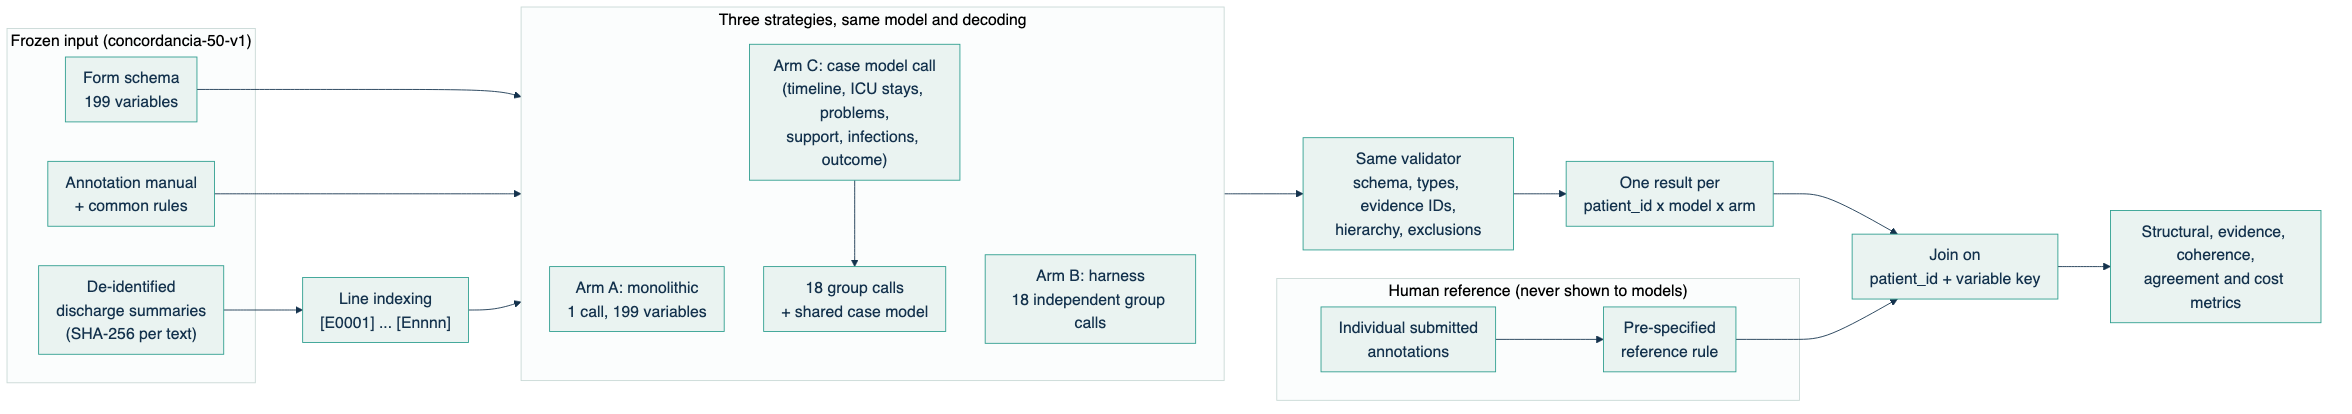
\includegraphics[width=\textwidth]{figuras/png/fig1_study_architecture.png}
\caption{\textbf{Study architecture.} The three arms receive the same frozen, line-indexed note, the same
schema and the same rules, run with the same model and decoding, and their outputs pass through the same
validator. Arm~C adds one call that builds a case model shared by its 18 group calls. The human reference is
stored and processed separately and is joined only after inference, on \texttt{patient\_id} and
variable key. Source: \texttt{form199\_v1} code and the 23 September 2026 snapshot.}
\label{fig:architecture}
\end{figure}

\begin{figure}[p]
\centering
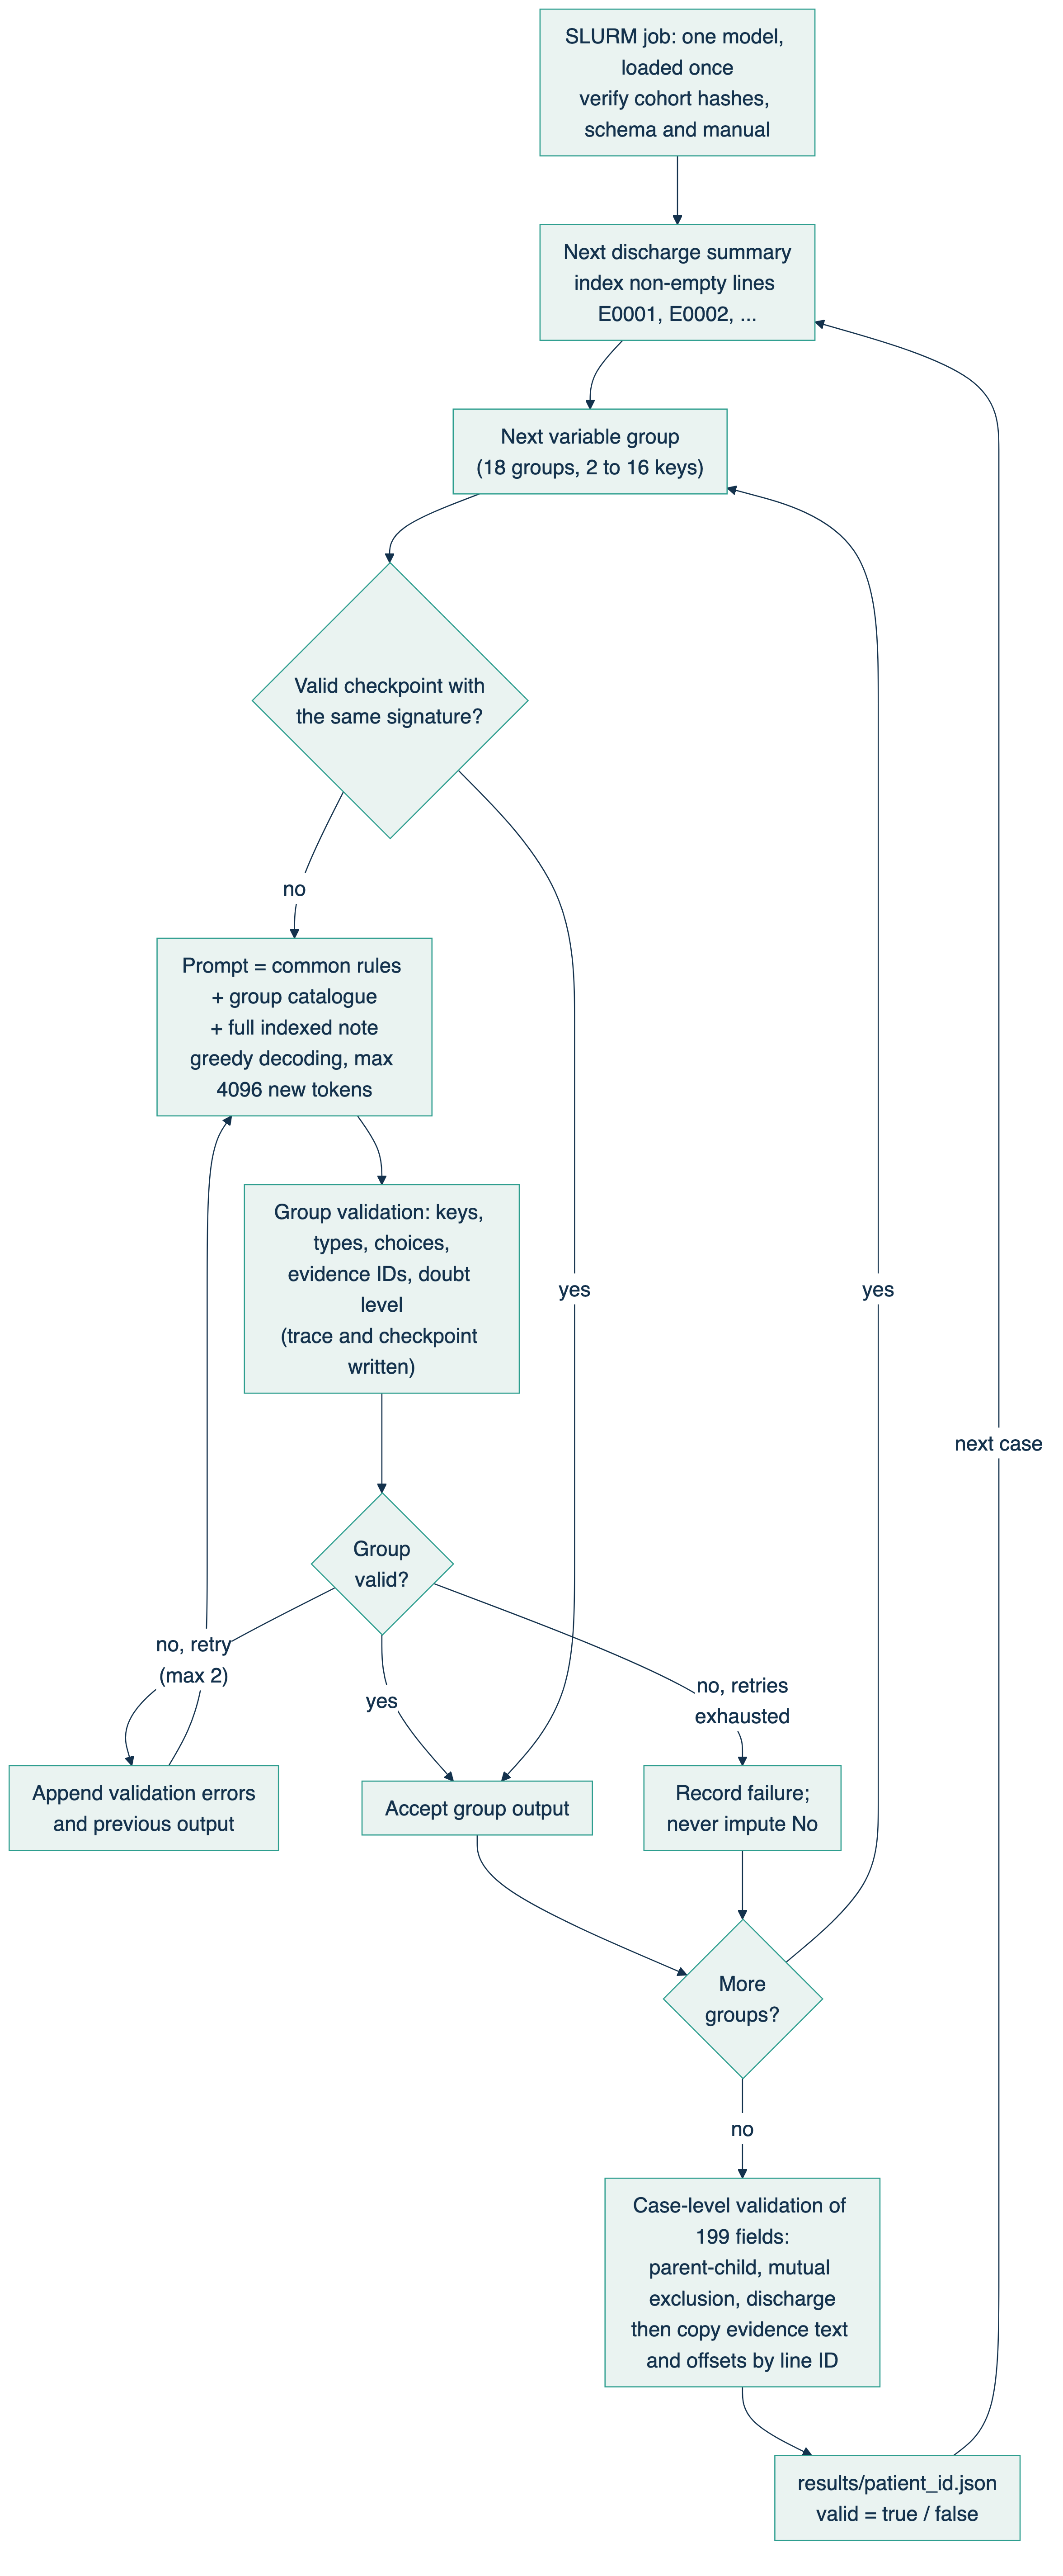
\includegraphics[height=0.86\textheight]{figuras/png/fig2_harness_flow.png}
\caption{\textbf{Arm B: multi-call harness.} For each case, 18 group calls are issued over the full note.
Each group output is validated immediately and retried at most twice with the errors and previous output;
a group that remains invalid is recorded as failed and is never imputed as No. Cross-group relations are
validated once all groups are merged. Evidence text and offsets are copied from the note by line
identifier. Traces and signed checkpoints allow resumption without repeating validated groups.}
\label{fig:harness}
\end{figure}

\begin{figure}[p]
\centering
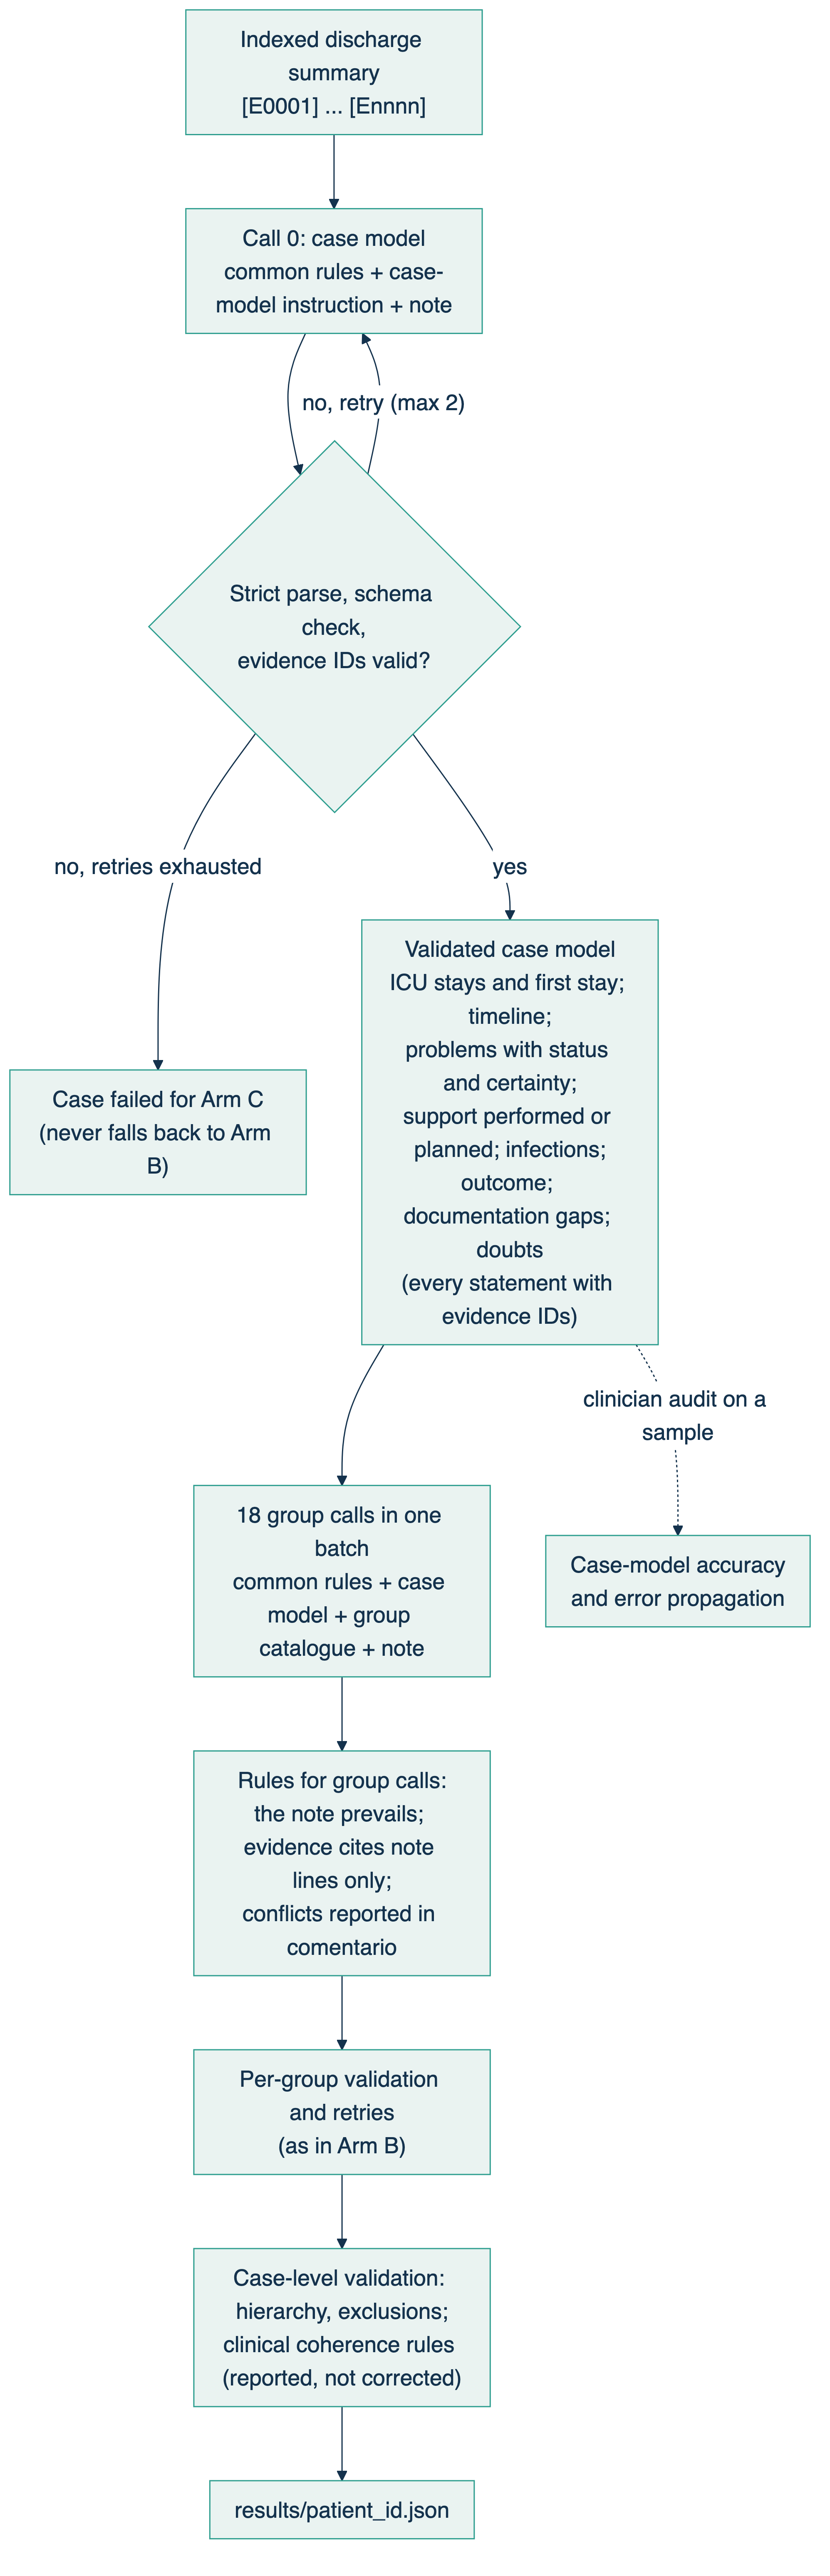
\includegraphics[height=0.82\textheight]{figuras/png/fig2b_arm_c.png}
\caption{\textbf{Arm C: harness with a shared case model.} A first call builds an evidence-grounded model of
the episode (ICU stays, timeline, problem status, support, infections, outcome, documentation gaps), validated
like any other output. The 18 group calls of Arm~B then run in one batch with the case model added to their
prompts; the note prevails in any conflict and evidence must cite note lines. A case whose case model remains
invalid is recorded as failed for Arm~C. A clinician audits the case model on a sample to measure accuracy and
error propagation.}
\label{fig:armc}
\end{figure}

\begin{table}[tbp]
\centering\small
\caption{\textbf{Variable groups of Arm B.} Groups follow form order within each block; the partition is
mechanical (at most 16 consecutive variables per block). Source: \texttt{manifest.json} and
\texttt{form\_schema.json} (\formv{}).}
\label{tab:groups}
\begin{tabular}{lrrrrr}
\toprule
Group & Variables & Boolean & Date & Select & Text \\
\midrule
hospitalizacion\_01 & 2 & 0 & 2 & 0 & 0 \\
antecedentes\_01 & 16 & 16 & 0 & 0 & 0 \\
antecedentes\_02 & 16 & 16 & 0 & 0 & 0 \\
antecedentes\_03 & 16 & 16 & 0 & 0 & 0 \\
antecedentes\_04 & 16 & 16 & 0 & 0 & 0 \\
antecedentes\_05 & 7 & 7 & 0 & 0 & 0 \\
ingreso\_01 & 4 & 0 & 1 & 1 & 2 \\
soporte\_01 & 16 & 13 & 0 & 1 & 2 \\
soporte\_02 & 16 & 7 & 7 & 0 & 2 \\
soporte\_03 & 16 & 15 & 0 & 0 & 1 \\
soporte\_04 & 9 & 9 & 0 & 0 & 0 \\
falla\_01 & 9 & 9 & 0 & 0 & 0 \\
infecciones\_01 & 16 & 16 & 0 & 0 & 0 \\
infecciones\_02 & 16 & 16 & 0 & 0 & 0 \\
infecciones\_03 & 10 & 10 & 0 & 0 & 0 \\
complicaciones\_01 & 7 & 7 & 0 & 0 & 0 \\
egreso\_01 & 5 & 1 & 1 & 2 & 1 \\
calidad\_01 & 2 & 0 & 0 & 1 & 1 \\
\midrule
Total (18 groups) & 199 & 174 & 11 & 5 & 9 \\
\bottomrule
\end{tabular}
\end{table}

\begin{table}[tbp]
\centering\small
\caption{\textbf{Reproducible configuration of models and hardware.} Read from the model configuration
files and from the log of each job (library versions, GPUs, driver and code hashes).}
\label{tab:models}
\footnotesize
\begin{tabularx}{\textwidth}{>{\raggedright\arraybackslash}p{0.2\textwidth}YYY}
\toprule
 & Gemma 4 & Llama 3.3 & Qwen 3.6 \\
\midrule
Checkpoint & \texttt{google/\allowbreak gemma-4-31B-it} & \texttt{meta-llama/\allowbreak Llama-3.3-\allowbreak 70B-Instruct} & \texttt{Qwen/\allowbreak Qwen3.6-\allowbreak 35B-A3B} \\
Architecture (config) & \texttt{Gemma4For\allowbreak Conditional\allowbreak Generation} & \texttt{LlamaFor\allowbreak CausalLM} & \texttt{Qwen3\_5Moe\allowbreak For\allowbreak Conditional\allowbreak Generation} (mixture of experts) \\
Local snapshot (SHA-256 of \texttt{config.json}, first 16 hex) & \texttt{e967dd38bc5cfd38} & \texttt{95ef9768e4741543} & \texttt{93a4693fa9d8392f} \\
Context window (config) & 262{,}144 & 131{,}072 & 262{,}144 \\
Precision & \multicolumn{3}{p{0.7\textwidth}}{4-bit NF4, double quantisation, bfloat16 compute (loader rule: GPU memory 47.4 GiB $<$ 60 GB)} \\
Instruction placement & user turn & system turn & system turn \\
Decoding & \multicolumn{3}{p{0.7\textwidth}}{greedy; reasoning mode off; stop at first complete JSON object; chunked prefill (1{,}024 tokens); corrected sliding-window cache for Gemma~4} \\
Max new tokens & \multicolumn{3}{p{0.7\textwidth}}{Arm B: 4{,}096 per call; Arm A: 16{,}384 (sensitivity: 4{,}096)} \\
Retries & \multicolumn{3}{p{0.7\textwidth}}{up to 2 per group (Arm B) or per form (Arm A)} \\
\midrule
Hardware & \multicolumn{3}{p{0.7\textwidth}}{1 node, SLURM batch partition; 2 $\times$ NVIDIA RTX A6000 (48 GB); 10 CPU cores; 64 GB RAM; driver 580.173.02} \\
Software & \multicolumn{3}{p{0.7\textwidth}}{Python 3.11.15; PyTorch 2.5.1 (CUDA 12.1); Transformers 5.5.4; bitsandbytes 0.49.2; Accelerate 1.14.0} \\
Code (SHA-256, first 12 hex) & \multicolumn{3}{p{0.7\textwidth}}{\texttt{runner.py} 4171537a9831; \texttt{protocol.py} 05d25791d35a; \texttt{monolithic.py} 8f665076a6e0; inference module 0e55f43baf86 \todoauthor{commit once versioned in git}} \\
\bottomrule
\end{tabularx}
\end{table}

\section{Results}\label{sec:results}

\noindent\emph{Status of this section.} Measured so far: the cohort description, the human annotation, the
offline verification of the pipeline, an eligibility and de-identification screen, and a single-case pilot of
Arms A and B with Gemma~4. Arm~C has not been run. Every comparative result is marked as pending and is
accompanied by the analysis that will produce it.

\subsection{Data flow}

Of the 275 de-identified summaries in the platform, 50 form the frozen cohort (\cref{fig:flow}). All
50 were planned for three independent annotations (150 assignments across six reviewers). At the data
cut of 23 September 2026, 63 annotations had been submitted by four reviewers: 7 summaries had no
submission, 24 had one, 18 had two and 1 had three. Forty-three summaries therefore have at least one
human annotation and 19 have at least two. All 50 summaries enter the structural, evidence and cost
analyses, which do not require a human reference.

\paragraph{Eligibility and de-identification screen.} The header of each summary records the units of
admission and discharge of the hospitalisation: 16 summaries started and 20 ended in the adult ICU, and the
rest started or ended in surgical, medical, intermediate-care, emergency or recovery units, which is
compatible with an ICU stay in the middle of the hospitalisation. A lexical screen found no mention of the
ICU, the high-dependency unit or intensive care in 12 of the 50 summaries; these are candidates for
exclusion from the agreement analyses, pending clinical review (Section~\ref{sec:setting}). The same screen
found the hospital record number unmasked in the header of 12 summaries, which led to the corrected
redaction and the re-export of 24 September 2026 (Section~\ref{sec:setting}); the annotation counts in this
section still refer to the 23 September cut. These counts come from a pattern search on the model
input and are reported without any identifier.

\begin{figure}[tbp]
\centering
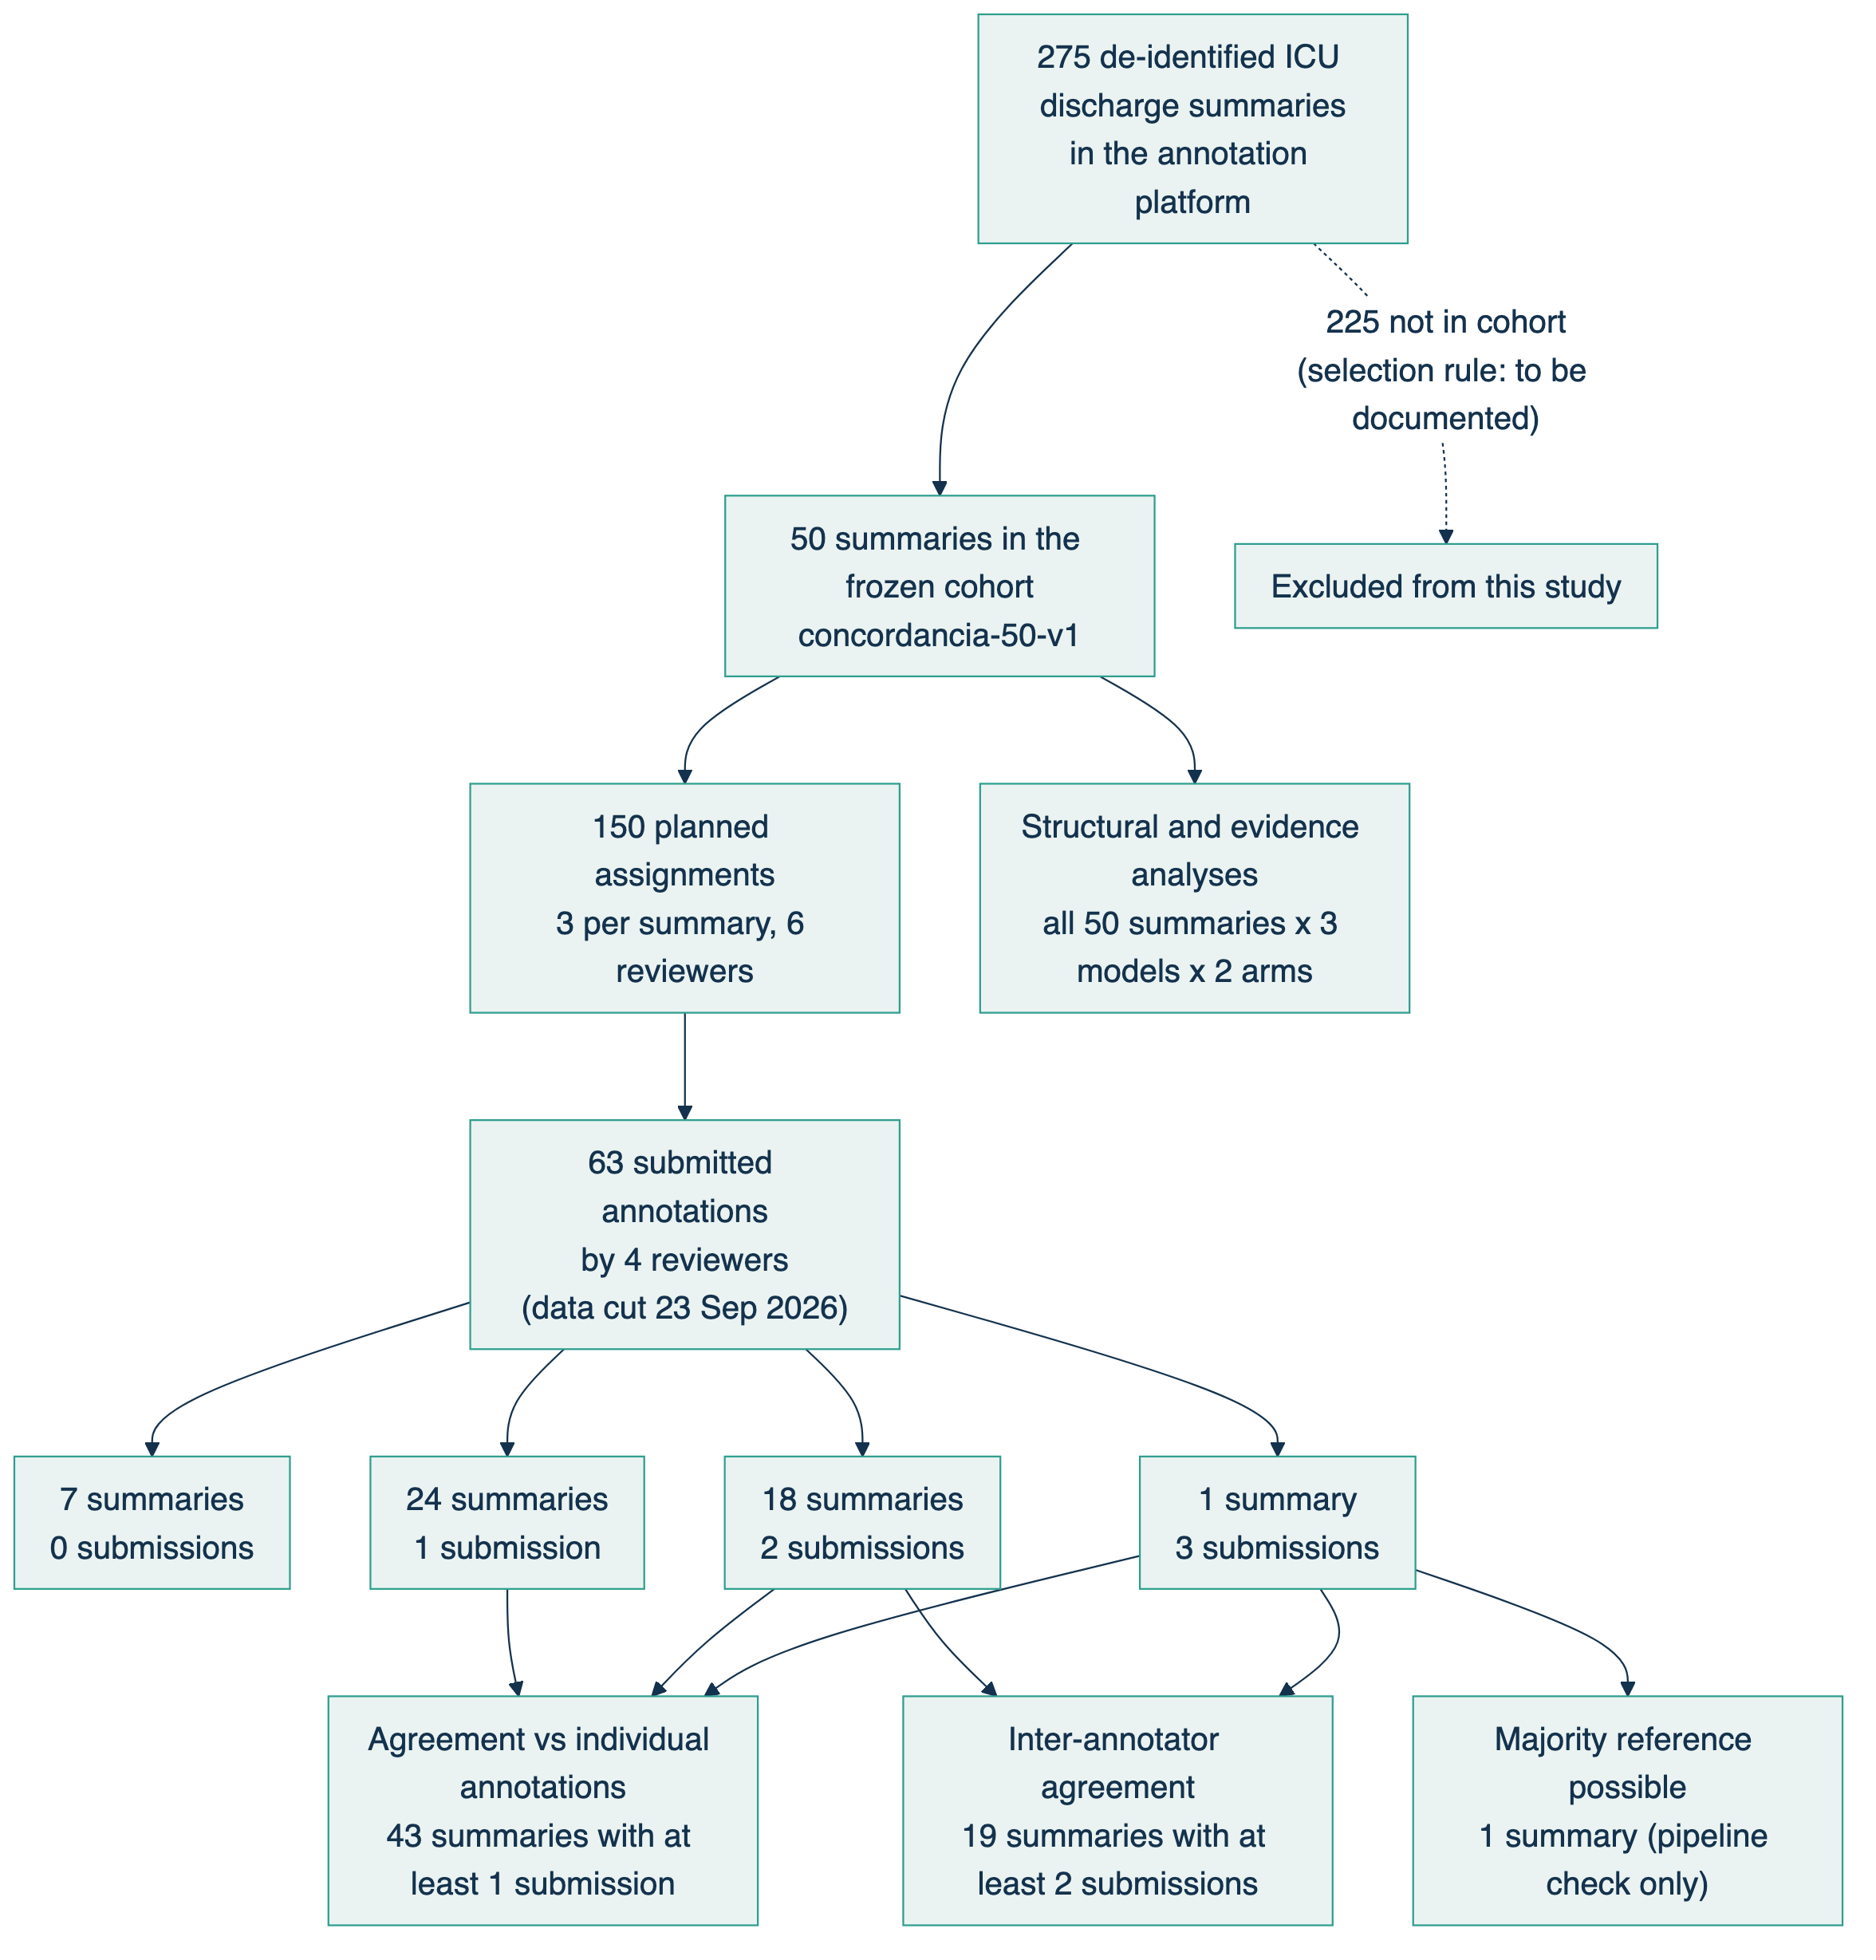
\includegraphics[width=0.78\textwidth]{figuras/png/fig3_inclusion.png}
\caption{\textbf{Inclusion and analysis sets.} Counts from the 23 September 2026 snapshot
(\texttt{snapshot.json}, \texttt{assignments.json}, \texttt{submitted\_annotations.json}). Unit: discharge
summary. Submissions are counted per summary; unsubmitted assignments are not treated as negative
annotations. The selection rule from 275 to 50 summaries is pending documentation.}
\label{fig:flow}
\end{figure}

\subsection{Cohort characteristics}

\Cref{tab:cohort} describes the cohort and the annotation workload. Summaries had a median of 3 pages
(IQR 2--3.25; range 2--6), 168.5 text spans (IQR 128--229) and 6{,}048.5 characters (IQR 3{,}270--8{,}722;
range 1{,}628--15{,}628), which yield a median of 115 indexed non-empty lines per note (range 50--303).
Clinical and demographic characteristics are not part of the model input and are not reported here
\todoauthor{decide whether aggregate age, sex, ICU length of stay and ICU mortality can be reported from
the platform's clinical data without re-identification risk}.

\begin{table}[tbp]
\centering\small
\caption{\textbf{Cohort characteristics and annotation workload.} Source:
\texttt{documents\_manifest.json}, \texttt{notes.jsonl} and the reference files of the 23 September 2026
snapshot, summarised by \texttt{scripts/cohort\_aggregates.py}. IQR, interquartile range.}
\label{tab:cohort}
\begin{tabularx}{\textwidth}{Yr}
\toprule
Characteristic & Value \\
\midrule
\multicolumn{2}{l}{\emph{Documents (unit: discharge summary, n = 50)}} \\
Pages, median (IQR) [range] & 3 (2--3.25) [2--6] \\
PDF text spans, median (IQR) [range] & 168.5 (128--229.25) [89--362] \\
Characters, median (IQR) [range] & 6{,}048.5 (3{,}270--8{,}721.75) [1{,}628--15{,}628] \\
Indexed non-empty lines, median (IQR) [range] & 115 (79.25--154.25) [50--303] \\
Total pages / spans / characters & 144 / 9{,}089 / 311{,}260 \\
\midrule
\multicolumn{2}{l}{\emph{Form}} \\
Answerable variables (boolean / date / select / text) & 199 (174 / 11 / 5 / 9) \\
Mother categories (context only, not scored) & 23 \\
Variables with a boolean ancestor / with mutual exclusions & 96 / 8 \\
\midrule
\multicolumn{2}{l}{\emph{Human annotation (data cut 23 Sep 2026)}} \\
Planned assignments (3 per summary; reviewers) & 150 (6) \\
Submitted annotations (reviewers submitting) & 63 (4) \\
Summaries with 0 / 1 / 2 / 3 submissions & 7 / 24 / 18 / 1 \\
Boolean items matched to the form: Yes / No / ? / unanswered & 1{,}189 / 9{,}729 / 0 / 43 \\
Yes answers per submission, median (IQR) [range] & 18 (10--25) [2--43] \\
Yes answers with captured evidence text & 1{,}183 of 1{,}189 \\
Boolean variables never marked Yes in any submission & 40 of 174 \\
\bottomrule
\end{tabularx}
\end{table}

\subsection{Quality of the human annotation}\label{sec:res-annotation}

Across the 63 submissions, 10{,}961 of the expected 10{,}962 boolean items could be matched to the form; in one
submission the key of one variable had been partially masked by the de-identification step during export, and that
item is excluded rather than re-mapped by hand. Of the matched items, 1{,}189 were Yes (10.8\%), 9{,}729 No and 43
left unanswered in 26 submissions. No reviewer used the ? option. Six of the 1{,}189 Yes answers lacked
captured evidence text despite the manual's requirement. Forty of the 174 boolean variables were never
marked Yes in any submission, so per-variable sensitivity and F1 are undefined for them with the current
data.

Agreement between reviewers was estimated on 19 summaries with at least two submissions, giving 21 pairs of
submissions and 3{,}616 item pairs after excluding 38 pairs with an unanswered item (\cref{tab:iaa}). Observed
agreement was 0.946 and pooled Cohen's $\kappa$ was 0.76 (95\% CI 0.70--0.82). Agreement on the presence of
a finding was lower than on its absence: positive specific agreement was 0.79 (95\% CI 0.73--0.84) and
negative specific agreement 0.97. Agreement varied by block, from $\kappa = 0.85$ for medical history to
$\kappa = 0.54$ for complications and $0.64$ for infections; the discharge block contributed only 21 item pairs.
These figures describe reviewer agreement at the data cut; they are not an estimate of model performance.
They are not directly comparable with an earlier summary produced by the platform's agreement panel on a
15 September cut (mean $\kappa$ 0.72), which averages per-criterion $\kappa$ over the 222 nodes of the form, including
mother categories, and used an earlier set of submissions.

\begin{table}[tbp]
\centering\small
\caption{\textbf{Inter-annotator agreement on the 174 boolean variables.} Unit: pair of submissions for the
same summary $\times$ variable, unanswered items excluded. $\kappa$ is Cohen's kappa pooled over item pairs;
PSA and NSA are positive and negative specific agreement. 95\% CIs from 5{,}000 case-level bootstrap
replicates (seed 20260923). Source: \texttt{datos/cohort\_aggregates.json}.}
\label{tab:iaa}
\begin{tabular}{lrrrr}
\toprule
Block & Item pairs & Observed agreement & $\kappa$ & PSA \\
\midrule
Medical history & 1{,}471 & 0.978 & 0.850 & 0.862 \\
Support and interventions & 919 & 0.940 & 0.788 & 0.824 \\
Organ failure & 186 & 0.866 & 0.711 & 0.818 \\
Infections & 874 & 0.927 & 0.642 & 0.683 \\
Complications & 145 & 0.890 & 0.537 & 0.600 \\
ICU discharge & 21 & 0.905 & 0.611 & 0.667 \\
\midrule
\makecell[l]{All boolean variables\\(19 summaries, 21 pairs)} & 3{,}616 & 0.946 & \makecell[r]{0.761\\(0.695--0.819)} & \makecell[r]{0.791\\(0.732--0.843)} \\
\bottomrule
\end{tabular}
\end{table}

\subsection{Pipeline verification}

Offline verification without inference confirmed that the generated prompts match the protocol hash, that
the catalogue contains exactly 199 unique variables in 18 groups, and that the 50 texts, the schema and the
manual match the frozen snapshot. Fifteen unit tests on synthetic notes, covering the output contract, evidence
identifiers and offsets, missingness reasons, parent--child and exclusion checks, resumption from checkpoints and
the rule that an incomplete response is never converted into No,
passed on the development machine and on the cluster within a SLURM allocation. These checks establish that
the pipeline behaves as specified on synthetic inputs; they say nothing about extraction quality.

\subsection{Pilot run}\label{sec:res-pilot}

The pilot processed the first summary of the cohort with Arms A and B and Gemma~4 under version~1.2
(\cref{tab:pilot}). On inspection, the summary described a two-day elective surgical admission without an ICU
stay, so it tests the pipeline but not the extraction of ICU variables. Both arms returned all 199 variables
with well-formed values, no truncation and valid evidence identifiers whose copied text matched the note in
every case. Arm~B needed one retry in 2 of its 18 groups; its merged output violated 6 parent--child relations,
all involving 3 non-boolean fields of invasive ventilation that one group answered as undocumented while
another group had answered that ventilation did not occur, which the protocol requires to be recorded as not
applicable. Arm~A was invalid on its first attempt (3 errors, one of them a parent--child violation within the
form) and valid after one retry. The two arms disagreed on 9 of 199 values: 4 medical-history variables and 5
ICU admission and discharge variables, which Arm~A filled from the hospitalisation while Arm~B left them empty.
Generation took 39~min in Arm~B and 3~h~47~min in Arm~A, whose single prompt of 42{,}091 tokens was decoded at
about 2 tokens per second. Earlier versions of Arm~B on the same case (versions 1 and 1.1) produced raw
responses identical to version~1.2 in all 20 calls. These observations concern one ineligible case; they are
reported as pipeline checks and carry no inferential weight.

\begin{table}[tbp]
\centering\small
\caption{\textbf{Pilot run, one summary without ICU stay, Gemma~4, version 1.2.} Source:
\texttt{datos/pilot\_v12\_gemma4.json} (aggregates without identifiers), from the traces of jobs 98635 and 98636.
Engine: Transformers with 4-bit NF4 on two RTX A6000 GPUs. No confidence intervals.}
\label{tab:pilot}
\begin{tabular}{lrr}
\toprule
 & Arm A (monolithic) & Arm B (harness) \\
\midrule
Case valid after retries & yes & no (6 relation errors) \\
Variables with a valid answer & 199/199 & 199/199 \\
Calls (retries) & 2 (1) & 20 (2) \\
Units valid at first attempt & 0/1 & 16/18 \\
Truncated calls & 0 & 0 \\
Raw responses bare / fenced / rejected & 0 / 2 / 0 & 0 / 20 / 0 \\
Input / output tokens & 93{,}939 / 25{,}485 & 104{,}648 / 14{,}831 \\
Generation time & 13{,}617 s & 2{,}331 s \\
Median output tokens per second & 1.9 & 6.4 \\
Peak GPU memory (both GPUs) & 50.2 GB & 22.1 GB \\
Boolean answers Yes / No / ? & 4 / 170 / 0 & 6 / 168 / 0 \\
Evidence items (offsets matching the note) & 14 (14) & 10 (10) \\
\bottomrule
\end{tabular}
\end{table}

\subsection{Structural validity (H1)}

\begin{resultspending}
\textbf{Table 3 (structural block).} For each model and arm: complete valid cases (/50); variable-level validity
(/9{,}950 patient--variable pairs); truncated calls and cases; omitted fields; parse outcome per call (bare, fenced, rejected) and offline
tolerant-parser sensitivity; the same outcomes on the first attempt only (sensitivity without retries); and Arm A with the
4{,}096-token budget. Differences B $-$ A with paired patient-level bootstrap 95\% CI and Holm-adjusted $p$.
\end{resultspending}

\subsection{Evidence fidelity (H2)}

\begin{resultspending}
Identifier validity (/identifiers returned), evidence coverage (/Yes and ? answers), evidence support in the
blinded review sample, and overlap with reviewer spans (/items where model and reviewer both answer Yes), by arm
and model, with paired differences and 95\% CI.
\end{resultspending}

\begin{figure}[tbp]
\begin{resultspending}[title={Figure 5 --- Evidence fidelity (RESULTS\_PENDING)}]
Grouped bars or dot plot: identifier validity, evidence coverage and evidence support, by model (panels) and arm
(colour), with 95\% CI. Denominators printed under each bar. Illustrative citation errors, if shown, must be
synthetic or fully redacted paraphrases approved by the clinical reviewers; no source text.
\end{resultspending}
\caption{Evidence fidelity by model and strategy. Source: \texttt{results/*.json} and the evidence-review form.}
\label{fig:evidence}
\end{figure}

\subsection{Agreement with human annotators (H3)}

\begin{resultspending}
\textbf{Table 3 (agreement block).} For the 174 boolean variables and each reference definition (individual,
43 summaries; concordant, 19 summaries): positive-class F1 (primary), accuracy, sensitivity, specificity,
balanced accuracy, PPV, MCC and Cohen's $\kappa$, with the model's ? handled as error and as abstention; the rate of
? per arm and model; macro-averages over variables with enough positive labels. Non-inferiority of B versus A per
model: difference in F1 with paired bootstrap 95\% CI against the margin $-\delta$.
\end{resultspending}

\begin{figure}[tbp]
\begin{resultspending}[title={Figure 4 --- Agreement by model and strategy (RESULTS\_PENDING)}]
Forest plot of positive-class F1 (point and 95\% CI) for Arm A and Arm B within each model, overall and by block,
with the difference B $-$ A and the non-inferiority margin shown as a vertical line. Unit: patient--variable pair;
resampling unit: patient; reference: individual annotations (43 summaries).
\end{resultspending}
\caption{Agreement with human annotators by model, strategy and block. Source: model results joined with
\texttt{submitted\_annotations.json} by \texttt{patient\_id} and variable key.}
\label{fig:agreement}
\end{figure}

\subsection{Cost and operational stability (H4)}

\begin{resultspending}
Per case and arm: calls, input and output tokens, latency (median, IQR), GPU-hours and peak GPU memory; retry rate
and recovery after retry; run-to-run identity in the repeatability subset.
\end{resultspending}

\begin{figure}[tbp]
\begin{resultspending}[title={Figure 6 --- Operational cost (RESULTS\_PENDING)}]
Small multiples by model: calls per case, input tokens per case, output tokens per case, latency per case and
GPU-hours for the cohort, Arm A versus Arm B, as paired dot plots (one line per case). Unit: case; denominators: 50
cases per arm and model.
\end{resultspending}
\caption{Operational cost by model and strategy. Source: inference metadata in trace files.}
\label{fig:cost}
\end{figure}

\subsection{Errors}

\begin{resultspending}
\textbf{Table 4.} Error taxonomy (\ref{app:errors}) of disagreements with the concordant reference, by arm
and model; parent--child and mutual-exclusion violations; and ablations: without retries, and Arm A with the
per-call budget. An ablation replacing evidence identifiers with model-written quotations is optional and would
require a separate pre-specified protocol version.
\end{resultspending}

\section{Discussion}\label{sec:discussion}

\subsection{Principal findings}

\pending{Summarise the paired differences for H1--H4 by model, with their confidence intervals, without
ranking models and without extrapolating beyond this cohort and schema.} At the current data cut, the
measured results concern the reference rather than the models. Pairwise agreement between reviewers on
the 174 boolean variables was substantial overall ($\kappa=0.76$), but agreement on the presence of a
finding (positive specific agreement 0.79) was lower than on its absence, and agreement was lowest for
complications and infections, the blocks whose manual rules require the most interpretation (the
infection cascade, colonisation versus infection, the severity threshold of delirium). Any model
evaluated against this reference inherits that uncertainty, which bounds the agreement that can be
expected and argues for reporting results by block.

\subsection{Why decomposition may help}

Four mechanisms favour the harness, and each maps onto a measured outcome. First, each call produces a
short output, so the risk of reaching the token limit falls (H1). Second, validation is local: an error
invalidates one group of at most 16 variables rather than the whole form, and the retry receives a
short, specific error list (H1, retry recovery). Third, each prompt carries only the definitions of the
requested variables, so the model does not need to keep 199 definitions in view while generating
(H2, H3). Fourth, the harness is operationally robust: signed checkpoints allow a job interrupted by the
scheduler to resume without repeating validated groups, which matters on a shared cluster with wall-time
limits (H4).

\subsection{Why decomposition may hurt}

Decomposition also has costs and failure modes that this design is built to expose rather than to hide.
The note is repeated in all 18 prompts, so input tokens and prefill time grow roughly with the number of
groups (H4). Related variables are answered in separate calls: the infection cascade spans three groups, and
51 of the 137 parent--child relations of the form (affecting 44 variables) and 3 of its 7 mutual-exclusion
pairs cross group boundaries. The per-group retry cannot
repair such inconsistencies, which are detected only when the groups are merged; the harness therefore
may produce more case-level relation errors than a single call that sees the whole form. Each call is
also asked, in isolation, to look for a small set of findings, which could bias it toward positive
answers for rare variables, as observed with category-specific prompts in earlier
work~\cite{agrawal2022fewshot}; the error taxonomy includes an over-calling category to detect this. Finally,
the partition is mechanical, consecutive variables within a block, and was not optimised; a different
grouping could change the results in either direction.

\subsection{What a shared case model can and cannot add}

Arm~C is designed to keep the advantages of decomposition (short outputs, local validation, batching) while
restoring what independent calls lose: a common reading of the episode. Its expected benefit is concentrated
where the pilot and the literature locate the difficulty. In a two-stage pipeline on psychiatric discharge
summaries, an intermediate extraction of events and times improved over direct extraction mainly for the most
inferential feature, the onset of the first episode~\cite{psych2stage2026}; in cancer registry abstraction, a
multi-agent pipeline improved context-dependent variables such as tumour grade but not highly structured ones
such as TNM stage~\cite{cancerregistrymas2026}. H6 therefore expects gains in infections, organ failure,
complications and ICU discharge rather than in medical history, and larger gains in poorly documented notes,
where information is scattered across sections or must be inferred. The case model also makes explicit whether
an ICU stay occurred at all, which in Arm~B each group decided separately. The same studies caution that
decomposition redistributes performance rather than improving it uniformly: in the cancer registry study
short, standardised fields such as metastasis stage lost recall~\cite{cancerregistrymas2026}, and in the
psychiatric study the intermediate layer did not help simple counts~\cite{psych2stage2026}. Its main risk is
propagation. In document-level extraction, context injected into every chunk outperformed both no context and
a single static summary, but an erroneous shared structure performed worse than no structure at all, with F1
falling from 0.80 to 0.45~\cite{hisccg2026}; the designers of the first blackboard system similarly reported that
focusing the search on low-level hypotheses whose credibility ratings were insufficiently accurate was
ineffective and harmful~\cite{erman1980hearsay}. This is why the case model must cite the note, the groups must give priority to
the note, the case model is audited by a clinician, and propagated errors are a category of the error
taxonomy. \pending{interpret H5 and H6.}

\subsection{Evidence by line identifier}

Citing evidence by line identifier and copying the text in software removes one failure mode, the
fabricated or paraphrased quotation, in both arms. It does not guarantee that the cited line supports the
answer, and a line of a PDF-derived text can be too coarse (several findings on one line) or too fine (a
sentence split across visual lines, or a table flattened into lines). For this reason evidence fidelity
is measured as identifier validity, coverage and clinician-judged support, not as literal matching, which
holds by construction. \pending{interpret H2 results.}

\subsection{Relation to previous work}

The direct comparisons available in the literature point in different directions and should not be read
as a general rule. Splitting a note into sentences raised F1 substantially over a single whole-document call
for dense entity extraction, at about twice the GPU time~\cite{llmie2025}; a prompt graph of sequential
subtasks gave the largest mean gain over zero-shot prompting in a multilingual benchmark, at roughly eight
times the time per report of few-shot prompting~\cite{spaanderman2025structured}; and sequential prompting did
not outperform few-shot prompting for timeline extraction with a 7B model~\cite{fornasiere2024medical}. None of
these studies decomposed a fixed schema of this size by output groups, so they motivate the hypotheses but do
not predict the result. \pending{relate the measured differences to these findings.}

Building an intermediate representation before the final extraction also has precedents. Clinical pipelines
have extracted events and temporal information before predicting chart-level features~\cite{psych2stage2026}
or reconstructing patient timelines~\cite{clinicirca2026}, and a pathology workflow passed the metadata of a planning step to parallel field extractors, although
without testing whether that shared context helped~\cite{promptplanextract2026}. Outside medicine, blackboard architectures
coordinated independent specialists through a shared data structure~\cite{erman1980hearsay,nii1986blackboard},
an idea recently revived for multi-agent LLM systems~\cite{blackboardllm2025,blackboardmas2025}, and
Skeleton-of-Thought generates a plan first and expands its parts in parallel~\cite{skeletonofthought2024}, the
same computational pattern as Arm~C. What these works do not provide is a paired comparison, on the same
patients and schema, between a single call, independent decomposed calls and decomposed calls that share a
verified representation of the case.

Two observations from earlier work are specific enough to be tested here. Agrawal et al.\ found that prompts
specialised for one category tended to produce an answer even when none was present~\cite{agrawal2022fewshot};
if the harness behaves similarly, it should show more positive answers for rare variables than the monolithic
call, which the over-calling category of the error taxonomy and the per-block positive rates are designed to
detect. Hein et al.\ observed more major errors in reports with many items to extract and argued that success
depended on the clarity of the instructions~\cite{iterativerefine2025}; the instruction text here was derived
from the annotators' manual rather than refined against the reference, which avoids overfitting the prompts
to the reference but may leave ambiguities that only an error analysis will reveal.

Other design choices in the literature address the same problems by different means. Grammar-constrained
decoding guarantees well-formed JSON~\cite{privacy2024structured} and would remove parse failures from all
arms, which is why parse success is reported separately from content validity. Entity-anchored retrieval
reduces the input sent to each call~\cite{clinicalentityretrieval2024}; in the harness the full note is repeated
in every call, so input-side decomposition is a natural complement to the output-side decomposition studied
here. Line-numbered input for evidence has been used before~\cite{fornasiere2024medical}, and criterion-level
decisions with sentence locations have been used for trial matching~\cite{trialgpt2024}; the difference here is
that identifiers are validated, the quotation is copied by software and the support of the cited lines is
assessed by clinicians.

\subsection{Limitations}

The study has a single centre, a single language and a single form, and 50 summaries; results may not
transfer to other hospitals, note styles or schemas. The cohort was not screened for the presence of an ICU
stay, and about a quarter of the summaries may not document one; the agreement analyses are restricted to
eligible summaries, which reduces the sample. Arm~C and hypotheses H5 and H6 were added after the pilot; they
were specified before any comparison with the human reference, but they were motivated by pilot observations.
The evaluation engine may differ from the pilot engine in precision (FP8 instead of NF4) and in batching, so the
pilot is not a calibration of the evaluation run. The human reference was incomplete at the data cut,
reviewers did not use the ? option, and no adjudicated consensus exists; individual references attenuate
absolute agreement, although they affect both arms equally. Positive findings are infrequent and 40
boolean variables were never marked positive, so per-variable estimates are unstable or undefined. The
model input is PDF-derived text grouped into visual lines, which can disorder tables or columns;
de-identification relied on pattern-based redaction, which masked parts of clinical words in 3 of 655
redacted segments, including a sedative drug name. The two arms necessarily differ in their output budget
and in the length of their prompts; the pre-specified budgets and the sensitivity analysis at an equal
per-call budget address this but cannot remove it. Greedy decoding on GPUs may not be bit-reproducible,
especially when prompts are batched and kernels are not batch-invariant; the batch-invariant mode, the
equivalence test and the repeatability subset address this, but only on the cases tested. Three models were evaluated, each with one run; conclusions about other models or sampling
settings would require new runs. Finally, the paired design isolates the calling strategy but not its
components (grouping, retries, per-group validation); the ablations without retries address only one of
them.

\subsection{Implications}

\pending{State what the measured trade-off implies for the design of extraction pipelines for long clinical
forms, limited to the measured outcomes.} Independently of the results, the protocol illustrates reporting
practices that make such comparisons auditable: frozen inputs with hashes, evidence that cannot be
fabricated, failures that are never converted into negative findings, and a reference whose agreement and
missingness are reported before it is used.

\section{Conclusion}\label{sec:conclusion}

This study specifies and instruments a paired comparison of three ways of extracting a 199-variable ICU form
from Spanish discharge summaries with open-weight models on local infrastructure: a single call, an 18-call
schema-constrained harness, and the same harness sharing an evidence-grounded model of the case. All strategies share the note, rules, output contract and
validator; evidence is cited by line and copied by software; and failed or truncated answers are never
recorded as negative findings. At the current data cut, the human annotation shows substantial pairwise
agreement on boolean variables, lower for positive findings and for infections and complications than for
medical history. \pending{Conclusions on H1--H6 will be stated only from the pre-specified paired analysis,
for this cohort, schema and these three models.} The pipeline is a research instrument for structured data
abstraction; it has not been evaluated for, and is not intended for, clinical use.

\section*{Declarations}

\subsection*{Ethics, privacy and governance}\label{sec:ethics}
\todoauthor{state the ethics committee that approved or exempted the use of the de-identified discharge
summaries (committee, protocol number, date) and whether informed consent was waived.} Discharge summaries were
de-identified before loading into the annotation platform. Model inference ran only on institutional hardware with
locally stored weights; no clinical text was sent to external services or commercial APIs. The human annotations
were kept on a separate machine and never transferred to the inference cluster. Result files are written with
owner-only permissions. This manuscript reports aggregate figures only; it contains no clinical text, patient
identifiers, dates or reviewer identities, and any illustrative example must be synthetic or approved by the
clinical team as non-identifying.

\subsection*{Data availability}
The discharge summaries and human annotations are clinical data of a public hospital and cannot be shared publicly.
\todoauthor{describe the access route, if any, e.g.\ on reasonable request subject to institutional approval.}
Aggregate, non-identifying results, including the cohort descriptors and agreement statistics reported here
(\texttt{datos/cohort\_aggregates.json}), are released with the manuscript.

\subsection*{Code availability}
The protocol (\texttt{protocol.py}), runner, generated prompts, form schema, annotation manual, manifest with hashes,
SLURM launch script and unit tests are versioned in the project repository
\todoauthor{public URL and commit, or statement of availability}. The script that computes the cohort and agreement
aggregates is \texttt{scripts/cohort\_aggregates.py}.

\subsection*{Use of generative AI in manuscript preparation}
\todoauthor{declare any use of AI assistants in drafting or editing this manuscript, as required by the target
journal.}

\subsection*{Funding}
\todoauthor{funding sources.}

\subsection*{Competing interests}
\todoauthor{declare competing interests.}

\subsection*{Author contributions}
\todoauthor{CRediT roles.}

\subsection*{Acknowledgements}
\todoauthor{acknowledge the clinical annotators by role, and the computing infrastructure.}


\bibliographystyle{vancouver}
\bibliography{references,references_extra}

\clearpage
\appendix
\renewcommand{\thesection}{Appendix \Alph{section}}
\section{Prompts}\label{app:prompts}

The prompts are written in Spanish, the language of the notes and of the annotation manual. They contain no
patient data. The 18 group prompts are generated by \texttt{protocol.py} from the frozen form schema and are
versioned with the code; the runner refuses to start if a generated prompt differs from the protocol. Every
group prompt is the common instruction text below followed by the group catalogue. At inference time the
line-indexed note is sent in the user turn, preceded by \emph{``Analiza la siguiente nota clínica y devuelve el
JSON estructurado. NOTA CLÍNICA COMPLETA:''} and followed by \emph{``Responde SOLO con el JSON válido.''} On a
retry, the errors of the previous attempt and its output are appended to the instruction text.

\paragraph{A.1 Common instruction text (\texttt{common.md}), shared by all calls and by Arm A.}
\lstinputlisting{secciones/apendices/prompts/common.md}

\paragraph{A.2 Example of a complete group prompt (\texttt{falla\_01.md}, 9 organ-failure variables).} The
first part repeats A.1 and is omitted here; the group-specific part is shown.
\lstinputlisting[firstline=94]{secciones/apendices/prompts/falla_01.md}

\paragraph{A.3 Arm A prompt.} The text of A.1 with one sentence changed (\emph{``responde únicamente las claves del
grupo solicitado''} becomes \emph{``\ldots del formulario solicitado''}), followed by the heading \emph{``Formulario
completo''}, the catalogue of the 199 variables serialised in the same order and format as the concatenation of the
18 group catalogues, and a closing instruction to read the whole note (114{,}338 characters in total, generated by
\texttt{monolithic.py}; a unit test checks that its catalogue equals the concatenated group catalogues).

\paragraph{A.5 Arm C case model (proposed schema, to be frozen with the clinical team).}\label{app:casemodel}
The case model is a JSON object; every statement carries \texttt{evidence\_ids} that must exist in the note.
Dates use DD/MM/YYYY or \texttt{null} with a reason. The instruction text for call~0 \todoauthor{to be written
and reviewed with a clinician; file \texttt{prompts/case\_model.md}, schema \texttt{case\_model\_schema.json}}
asks for statements supported by the note only, marks inferred statements as such, and lists doubts instead of
resolving them.
\begin{lstlisting}
{"episodio": {"hubo_estadia_uci": true,
   "estadias_uci": [{"orden": 1, "ingreso": "DD/MM/AAAA", "egreso": "DD/MM/AAAA",
                     "origen": "...", "destino": "...", "evidence_ids": ["E0011"]}],
   "primera_estadia": 1},
 "linea_de_tiempo": [{"momento": "antes_uci | durante_primera_uci | despues", "dia_relativo": 2,
   "evento": "...", "tipo": "ingreso | soporte | infeccion | procedimiento | complicacion | traslado | egreso",
   "certeza": "afirmado | negado | sospecha_descartada | sospecha_no_resuelta", "evidence_ids": []}],
 "problemas": [{"problema": "...", "estado": "antecedente_cronico | agudo_del_episodio",
   "certeza": "...", "evidence_ids": []}],
 "soportes": [{"soporte": "...", "realizado": true, "inicio": null, "fin": null, "evidence_ids": []}],
 "infecciones": [{"diagnostico": "...", "sepsis": false, "foco": null, "germen": null,
   "tratamiento": null, "evidence_ids": []}],
 "desenlace_primera_uci": {"estado_vital": "...", "destino": "...", "evidence_ids": []},
 "calidad_documental": {"secciones_vacias": [], "abreviaturas": {}, "contradicciones": [],
   "no_documentado": []},
 "dudas": [{"tema": "...", "por_que": "...", "evidence_ids": []}]}
\end{lstlisting}

\paragraph{A.6 Statement added to each Arm C group prompt.} The case model is inserted after the instruction
text with a fixed preamble stating that it is a generated aid that may contain errors, that the note prevails,
that evidence identifiers must cite note lines, and that conflicts must be reported in \texttt{comentario}.

\paragraph{A.4 Output schema.} Each of the requested keys maps to exactly
\texttt{\{valor, evidence\_ids, incertidumbre, comentario, motivo\_nulo\}}. The frozen form schema
(\texttt{form\_schema.json}, file SHA-256 \texttt{455fb92f\ldots}) is distributed with the code.

\section{Pseudocode}\label{app:pseudocode}

The pseudocode summarises \texttt{runner.py} (Arm B) and the specification of Arm A. \textsc{Validate} with
\emph{relations=false} applies the field-level checks of Section~\ref{sec:harness}; with \emph{relations=true} it adds
parent--child, mutual-exclusion and discharge-destination checks.

\begin{lstlisting}[mathescape=true]
procedure RUN_ARM_B(case, model, settings)          # settings: max_new_tokens=4096, max_retries=2
    indexed_note, index <- INDEX_LINES(case.text)   # [E0001] ... ; keeps offsets
    sig <- HASH(protocol, runner, inference_code, case.id, case.text, model, settings)
    merged <- {} ; calls <- 0
    for group in GROUPS(schema, size=16):           # 18 groups, form order
        cp <- LOAD_CHECKPOINT(case.id, group)
        if cp exists:
            if cp.signature != sig: abort("configuration changed; use a new output directory")
            if VALIDATE(cp.output, group.fields, index, relations=false) is empty:
                merged <- merged $\cup$ cp.output ; continue
        prompt <- COMMON + CATALOGUE(group)
        errors <- [] ; output <- none
        for attempt in 0..settings.max_retries:
            p <- prompt if attempt = 0 else prompt + RETRY_BLOCK(errors, output)
            output, meta <- GENERATE(model, p, indexed_note, settings.max_new_tokens, greedy)
            calls <- calls + 1
            errors <- VALIDATE(output, group.fields, index, relations=false)
            WRITE_TRACE_AND_CHECKPOINT(sig, group, attempt, p, output, errors, meta)
            if errors is empty: break
        if errors is empty: merged <- merged $\cup$ output     # failed group: keys stay missing, never "No"
    final_errors <- VALIDATE(merged, all_fields, index, relations=true)
    WRITE_RESULT(case.id, model, valid = (final_errors is empty), final_errors,
                 annotations = COPY_EVIDENCE(merged, index), calls)

procedure RUN_ARM_A(case, model, settings_A)       # monolithic.py; settings_A.max_new_tokens=16384
    indexed_note, index <- INDEX_LINES(case.text)
    prompt <- COMMON_ALL + CONCAT(CATALOGUE(g) for g in GROUPS(schema, size=16))
    for attempt in 0..settings_A.max_retries:
        output, meta <- GENERATE(model, prompt (+ RETRY_BLOCK), indexed_note, settings_A.max_new_tokens, greedy)
        errors <- VALIDATE(output, all_fields, index, relations=true)
        WRITE_TRACE(...) ; if errors is empty: break
    kept <- keys of the last output whose entries pass field-level checks; others missing, never "No"
    WRITE_RESULT(case.id, model, valid = (errors is empty), errors, COPY_EVIDENCE(kept, index), calls)

procedure RUN_ARM_C(case, model, settings)          # planned; same settings as Arm B
    indexed_note, index <- INDEX_LINES(case.text)
    for attempt in 0..settings.max_retries:
        cm, meta <- GENERATE(model, COMMON + CASE_MODEL_INSTRUCTION (+ RETRY_BLOCK), indexed_note, budget_cm)
        errors <- VALIDATE_CASE_MODEL(cm, CASE_MODEL_SCHEMA, index)   # strict parse, schema, evidence IDs
        WRITE_TRACE(...) ; if errors is empty: break
    if errors not empty: WRITE_RESULT(case.id, model, valid=false, reason="case model invalid"); return
    prompts <- [COMMON + CASE_MODEL_PREAMBLE + cm + CATALOGUE(g) for g in GROUPS(schema, size=16)]
    outputs <- GENERATE_BATCH(model, prompts, indexed_note)            # one batch; retries per group as in Arm B
    ... identical to RUN_ARM_B from group validation onwards, plus:
    coherence_violations <- COHERENCE_RULES(merged)                  # reported, never corrected
    contradictions_with_cm <- COMPARE(merged, cm)                    # counted for the audit
\end{lstlisting}

Arm A keeps the field-level valid entries of an invalid form, whereas Arm B discards a whole invalid group.
Variable-level validity is therefore computed with the same field-level rule in both arms (Section~\ref{sec:mono}).

\section{TRIPOD-LLM checklist}\label{app:tripod}

Items and applicability codes are those of TRIPOD-LLM Table 2 and the abstract checklist (Table 3)
\cite{gallifant2025tripodllm}. The guideline text mentions 19 main items and 50 subitems; the printed Table 2
has 49 numbered rows, which are listed here. This study is classified as LLM methods (M, prompt engineering)
and LLM evaluation (E); it is not an evaluation in a healthcare setting (H) and involves no model
development (D). Information extraction is not a separate task category in TRIPOD-LLM; items for all tasks
are applied, and item 7a is reported although its task codes do not list extraction. Status: \textbf{R},
reported in this draft; \textbf{P}, partially reported or pending data; \textbf{NA}, not applicable (with reason).

{\footnotesize
\setlength{\tabcolsep}{4pt}
\begin{longtable}{>{\raggedright\arraybackslash}p{0.9cm}>{\raggedright\arraybackslash}p{6.1cm}>{\raggedright\arraybackslash}p{3.1cm}>{\raggedright\arraybackslash}p{0.9cm}>{\raggedright\arraybackslash}p{3.2cm}}
\toprule
Item & Topic (abridged) & Location & Status & Note \\
\midrule
\endfirsthead
\toprule
Item & Topic (abridged) & Location & Status & Note \\
\midrule
\endhead
1 & Title identifies LLM evaluation, task, population, outcome & Title & R & \\
2 & Abstract per TRIPOD-LLM for abstracts & Abstract & P & Results pending \\
3a & Healthcare context, rationale, existing approaches & \S\ref{sec:intro}, \S\ref{sec:related} & R & \\
3b & Target population, intended use, intended users (E, H) & \S\ref{sec:intro}, \S\ref{sec:conclusion} & R & Research abstraction; no clinical use \\
4 & Objectives, development vs.\ evaluation & \S\ref{sec:objectives} & R & \\
5a & Data sources per dataset and rationale & \S\ref{sec:methods} (Setting) & P & Selection rule 275$\to$50 pending \\
5b & Data points, distribution, languages, countries & \cref{tab:cohort} & R & Clinical descriptors pending decision \\
5c & Dates of oldest and newest text & --- & P & \todoauthor{admission date range, aggregated} \\
5d & Preprocessing and quality checks & \S\ref{sec:methods} (Setting) & R & Redaction, line grouping, hashes \\
5e & Missing and imbalanced data & \S\ref{sec:reference}, \S\ref{sec:outcomes} & R & Unanswered, not submitted, failures \\
6a & LLM name, version, last training date & \cref{tab:models} & P & Revisions and dates pending \\
6b & Development process (M, D) & \cref{tab:models} & P & Cite model cards; no fine-tuning \\
6c & Text generation: prompt engineering, consistency, seed, temperature, max tokens & \S\ref{sec:prompts}--\ref{sec:models} & R & $B_{\text{mono}}$ pending \\
6d & Initial and post-processed output & \S\ref{sec:prompts}, \S\ref{sec:harness} & R & Raw output kept in traces \\
6e & Classification thresholds (C, OF) & --- & NA & No probabilities or thresholds \\
7a & Output quality metrics and error types & \S\ref{sec:outcomes}, \ref{app:errors} & R & \\
7b & Relevance of metrics to downstream task (E, H) & \S\ref{sec:outcomes} & P & Expand in Discussion \\
7c & Outcome definition, computation, metrics (E, H) & \S\ref{sec:outcomes}, \ref{app:stats} & R & Local models; no API dates \\
7d & Assessor qualifications, instructions, agreement & \S\ref{sec:reference}, \S\ref{sec:outcomes} & P & Reviewer profile pending \\
7e & Comparison with other LLMs, humans, standards & \S\ref{sec:stats} & R & Within-model arm comparison \\
8a & Annotation guidelines with examples & \S\ref{sec:reference} & R & Manual versioned; share as supplement \\
8b & Number of annotators, multiply annotated share, IAA & \S\ref{sec:res-annotation}, \cref{tab:iaa} & R & At data cut \\
8c & Annotator background and experience & \S\ref{sec:reference} & P & \todoauthor{profile} \\
9a & Prompt design, curation, selection & \S\ref{sec:prompts}, \S\ref{sec:separation} & R & \\
9b & Data used to develop prompts & \S\ref{sec:separation} & R & Manual, schema, synthetic tests \\
10 & Preprocessing before summarisation (SS) & --- & NA & No summarisation task \\
11 & Instruction tuning or alignment (M, D) & --- & NA & None performed \\
12 & Compute (M, D, E) & \S\ref{sec:models}, \cref{fig:cost} & P & Measured after runs \\
13 & Ethics approval and consent & Declarations & P & \todoauthor{committee} \\
14a & Funding & Declarations & P & \\
14b & Conflicts of interest & Declarations & P & \\
14c & Protocol access (H) & \ref{app:stats} & R & Not H; plan provided anyway \\
14d & Registration (H) & --- & NA & Not H; \todoauthor{consider OSF registration} \\
14e & Data availability & Declarations & P & \\
14f & Code availability & Declarations & P & Public URL pending \\
15 & Patient and public involvement (H) & --- & NA & Not H; state no involvement \\
16a & Flow of documents and labels (E, H) & \cref{fig:flow} & R & \\
16b & Characteristics per source and split (E, H) & \cref{tab:cohort} & R & Single source, no split \\
16c & Clinical variables development vs.\ evaluation (E, H) & --- & NA & No development split \\
16d & Participants and events per analysis (E, H) & \cref{fig:flow}, \ref{app:stats} & P & Final counts at data cut \\
17 & Performance on pre-specified metrics & \S\ref{sec:results} & P & RESULTS\_PENDING \\
18 & LLM updating & --- & NA & No updating \\
19a & Interpretation incl.\ fairness and previous studies & \S\ref{sec:discussion} & P & \todoauthor{fairness: subgroup data not in input} \\
19b & Limitations, bias, uncertainty, generalisability & \S\ref{sec:discussion} & R & \\
19c & Data challenges: representation, missingness, bias (E, H) & \S\ref{sec:discussion} & R & \\
19d & Intended use, input, end-user, autonomy (E, H) & \S\ref{sec:conclusion} & R & Human review required \\
19e & Handling poor-quality input (E, H) & \S\ref{sec:harness} & R & Failures never imputed \\
19f & User interaction and expertise (E, H) & --- & P & Describe reviewer role in use \\
19g & Next steps & \S\ref{sec:discussion} & P & After results \\
\midrule
2a--2l & Abstract checklist: title, background, objectives, setting, data, LLM name/version, building steps (M, D), task, evaluation data and metrics, results, implications, registration (H) & Abstract & P & 2g NA (no building); 2j pending; 2l NA (not H) \\
\bottomrule
\end{longtable}
}

\paragraph{Other guidelines.} TRIPOD+AI~\cite{collins2024tripodai} was written primarily for non-generative prediction
models; it is used for general items (data, reference standard, blinding of assessors, availability).
CONSORT-AI~\cite{liu2020consortai} and SPIRIT-AI~\cite{rivera2020spiritai} apply to randomised trials and trial
protocols. Because this study is retrospective and non-interventional, they are used only as transparency references:
the AI system version (CONSORT-AI 5(i)), the handling of input data and of poor-quality input (5(ii)--5(iii)), the
analysis of performance errors (19; SPIRIT-AI 22) and the pre-specification of the analysis before outcomes are seen.

\section{Error taxonomy and matrix}\label{app:errors}

Disagreements between a model and the concordant reference are classified by two clinician reviewers blinded to
arm and model, using the categories below; a disagreement may receive more than one category. Inter-reviewer
agreement on the taxonomy is reported. Categories are defined from the annotation manual so that they map to its
rules.

\begin{table}[h]
\centering\small
\caption{Error categories.}
\begin{tabularx}{\textwidth}{lY}
\toprule
Category & Definition and example of rule involved \\
\midrule
Temporality: history vs.\ acute & A pre-existing condition coded as an acute event or vice versa (e.g.\ acute kidney injury
coded as chronic kidney disease). \\
Temporality: stay & Information from a later ICU stay or from the hospital discharge used for the first ICU stay. \\
Negation & A negated or ruled-out finding coded as Yes, or an affirmed finding coded as No. \\
Planned vs.\ performed & An indicated or planned intervention coded as performed. \\
Support vs.\ failure & Organ support used as sole evidence of organ failure. \\
Infection cascade & Fever, laboratory abnormality, colonisation or an isolated culture coded as infection without a
diagnosis. \\
Hierarchy & Violation of parent--child consistency or mutual exclusion. \\
Prevalence / over-calling & Positive answers for findings not documented, typically rare variables. \\
Evidence absent & Yes or ? without any valid evidence identifier. \\
Evidence incorrect & Evidence identifiers valid but lines do not support the answer. \\
Genuine ambiguity & The note supports more than one reading; reviewers judge the model answer defensible. \\
Reference error & On review, the human reference is judged incorrect (reported, not used to change the reference
without adjudication). \\
Case-model propagation & (Arm C) The group answer follows an incorrect statement of the case model. \\
Structural failure & Answer missing because of truncation, parse failure or an invalid group or form. \\
\bottomrule
\end{tabularx}
\end{table}

\begin{resultspending}[title={Error matrix (RESULTS\_PENDING)}]
Rows: categories above. Columns: model $\times$ arm. Cells: count and percentage of disagreements (denominator:
disagreements with the concordant reference for that model and arm). A second matrix cross-tabulates Arm A and Arm B
errors on the same patient--variable pairs (both correct, only A correct, only B correct, both wrong).
\end{resultspending}

\section{Statistical analysis plan}\label{app:stats}

This plan is to be registered, with date and commit, before model outputs of the evaluation run are joined with
the human reference. Any later change is reported as a deviation with its reason.

\paragraph{E.1 Analysis sets.} \emph{Structural set}: all cases $\times$ 3 models $\times$ 3 arms.
\emph{Eligible set}: summaries with a clinician-confirmed ICU stay; all agreement, coherence and H6 analyses use
it, and results on ineligible summaries are reported separately. \emph{Individual reference
set}: cases with at least one submitted annotation (43 at the data cut). \emph{Concordant reference set}: cases with at
least two submissions (19 at the data cut), items with full agreement. \emph{Pilot}: one case, descriptive only.
The analysis sets are recomputed at the final data cut, which is fixed \todoauthor{date} before joining.

\paragraph{E.2 Estimands.} For each model $m$ and outcome $Y$, the estimands are the paired differences
$\Delta^{BA}_m = Y_m^{B} - Y_m^{A}$ (primary), $\Delta^{CB}_m = Y_m^{C} - Y_m^{B}$ and $\Delta^{CA}_m = Y_m^{C} - Y_m^{A}$
(secondary) on the same cases. Proportions are computed on pooled patient--variable pairs (or calls, or evidence
identifiers, as stated per outcome) within the analysis set.

\paragraph{E.3 Confidence intervals.} Paired percentile bootstrap resampling cases with replacement (5{,}000
replicates, seed 20260923): in each replicate both arms are recomputed on the same resampled cases, preserving
pairing and within-case correlation. For the individual reference, each case's submissions stay together and each
case has equal weight. BCa intervals are reported as sensitivity if percentile intervals are asymmetric.

\paragraph{E.4 Hypothesis tests.} H1 and H2: two-sided test of $\Delta_m = 0$ via the bootstrap distribution, with
superiority of the decomposed arm claimed only if the 95\% CI excludes 0 in its favour. H3: non-inferiority, concluded if
the lower 95\% bound of $\Delta_m$ in positive-class F1 exceeds $-\delta$; superiority is assessed only after
non-inferiority. H4: estimation only. H5: superiority of C over B in coherence-rule violations per case. H6: superiority of C over
B in positive-class F1 within the inferential blocks, non-inferiority in medical history, and an arm-by-quality
interaction estimated in the mixed model of E.5 (C versus B, low versus other notes). Holm adjustment across
models and comparisons within each hypothesis; secondary outcomes are exploratory, unadjusted and labelled as
such.

\paragraph{E.5 Mixed-effects sensitivity analysis.} For binary item-level outcomes (valid, correct): logistic mixed
model $\text{logit}\,P(Y_{ijm}=1) = \beta_0 + \beta_1\,\text{arm} + u_i + v_j$ fitted per model, with random intercepts for
patient $i$ and variable $j$; reported if the model converges without separation. A pooled model with
$\text{arm}\times\text{model}$ interaction is descriptive.

\paragraph{E.6 Handling of missing and special values.} Missing answers from truncation or failure count as invalid
and, for agreement, as incorrect in the primary analysis; a complete-case sensitivity analysis restricted to pairs
answered by both arms is reported. Model ? is analysed as error and as abstention (Section~\ref{sec:outcomes}). Human
unanswered items and unsubmitted assignments are excluded, never treated as No.

\paragraph{E.7 Multiplicity and variables.} The 199 variables are not independent units; no per-variable hypothesis
tests are performed. Per-variable and per-block results are descriptive, shown with case-bootstrap CIs, and restricted
to variables with at least \todoauthor{k} positive reference labels.

\paragraph{E.8 Software.} Python \pending{version}; analysis code versioned with the protocol. \todoauthor{name the
repository path of the analysis script once written.}


\end{document}
